\chapter{Feature Extraction}\label{Ch:feature}
% \begin{document}


%\section{Feature Extraction}

\section{Fourier Transformation}
The Fourier transformation converts signals from spatial domain to frequency domain and vice verse. The two-dimensional Discrete Fourier Transform (DFT) is used to process two-dimensional discrete signals such as images \cite{Cooley}. Given a one-channel signal $f(x,y)$ with dimensions $M\times N$, its DFT $F(u,v)$ is given by
\begin{align}
F(u,v)=\frac{1}{\sqrt{MN}}\sum\limits_{x=0}^{M-1}\sum\limits_{y=0}^{N-1}f(x,y)e^{-2i\pi\frac{ux}{M}}e^{-2i\pi \frac{vy}{N}},
\end{align}
where $0\leqslant u\leqslant M-1$ and $0\leqslant v\leqslant N-1$ are the spectral coordinates \cite{Burger}. However, for visualization purposes, we shift the zero frequency $(0,0)$ to the center $(\frac{m}{2},\frac{n}{2})$ of the image so that $-\lfloor\frac{M}{2}\rfloor\leqslant u\leqslant \lfloor\frac{M-1}{2}\rfloor$ and $-\lfloor\frac{N}{2}\rfloor\leqslant v\leqslant \lfloor\frac{N-1}{2}\rfloor$. The original signal can be extracted from $F(u,v)$ with
\begin{align}
f(x,y)=\frac{1}{\sqrt{MN}}\sum\limits_{u=0}^{M-1}\sum\limits_{v=0}^{N-1}F(u,v)e^{2i\pi\frac{ux}{M}}e^{2i\pi \frac{vy}{N}}.
\end{align}
The rationale behind considering DFT as a feature for the graphics artifact classification is that several types of graphics (e.g. morse code, parallel lines, etc.) exhibit periodic patterns that could be best identified in the frequency domain. Previous studies provide evidence of successful application of this technique to the detection of periodic patterns in signals \cite{russians}. Additionally, most graphics corruptions have sharp edges and fine structure, which finds reflection in the high-frequency components. For example, Figures \ref{fig:fourier1}, \ref{fig:fourier2}, \ref{fig:fourier4} and \ref{fig:fourier3} show the Fourier transformation of the ``Borderlands 2'' game screenshot with different graphics artifacts added. Note that intensities represent log-transformed absolute values of the corresponding DFT descriptors.
\begin{figure}[H]
\centering
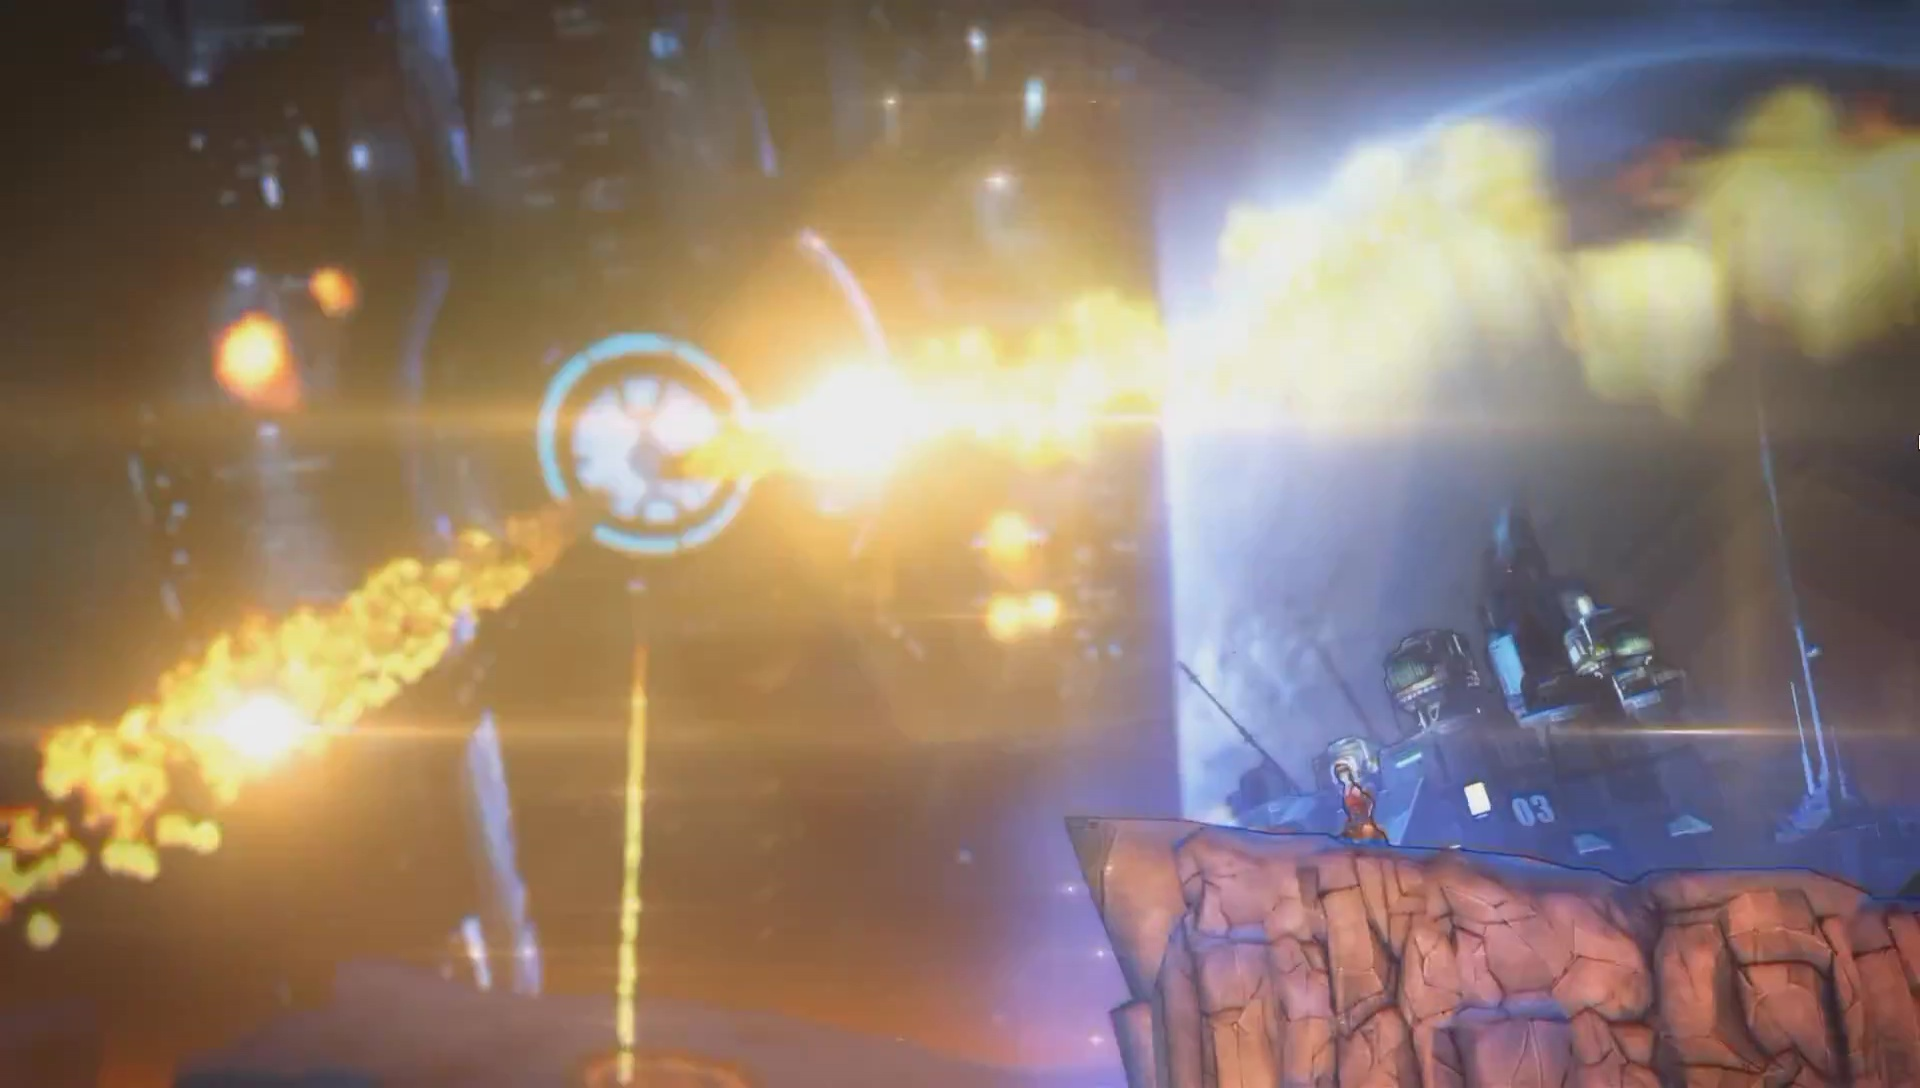
\includegraphics[scale=0.11]{images/bd.jpg}
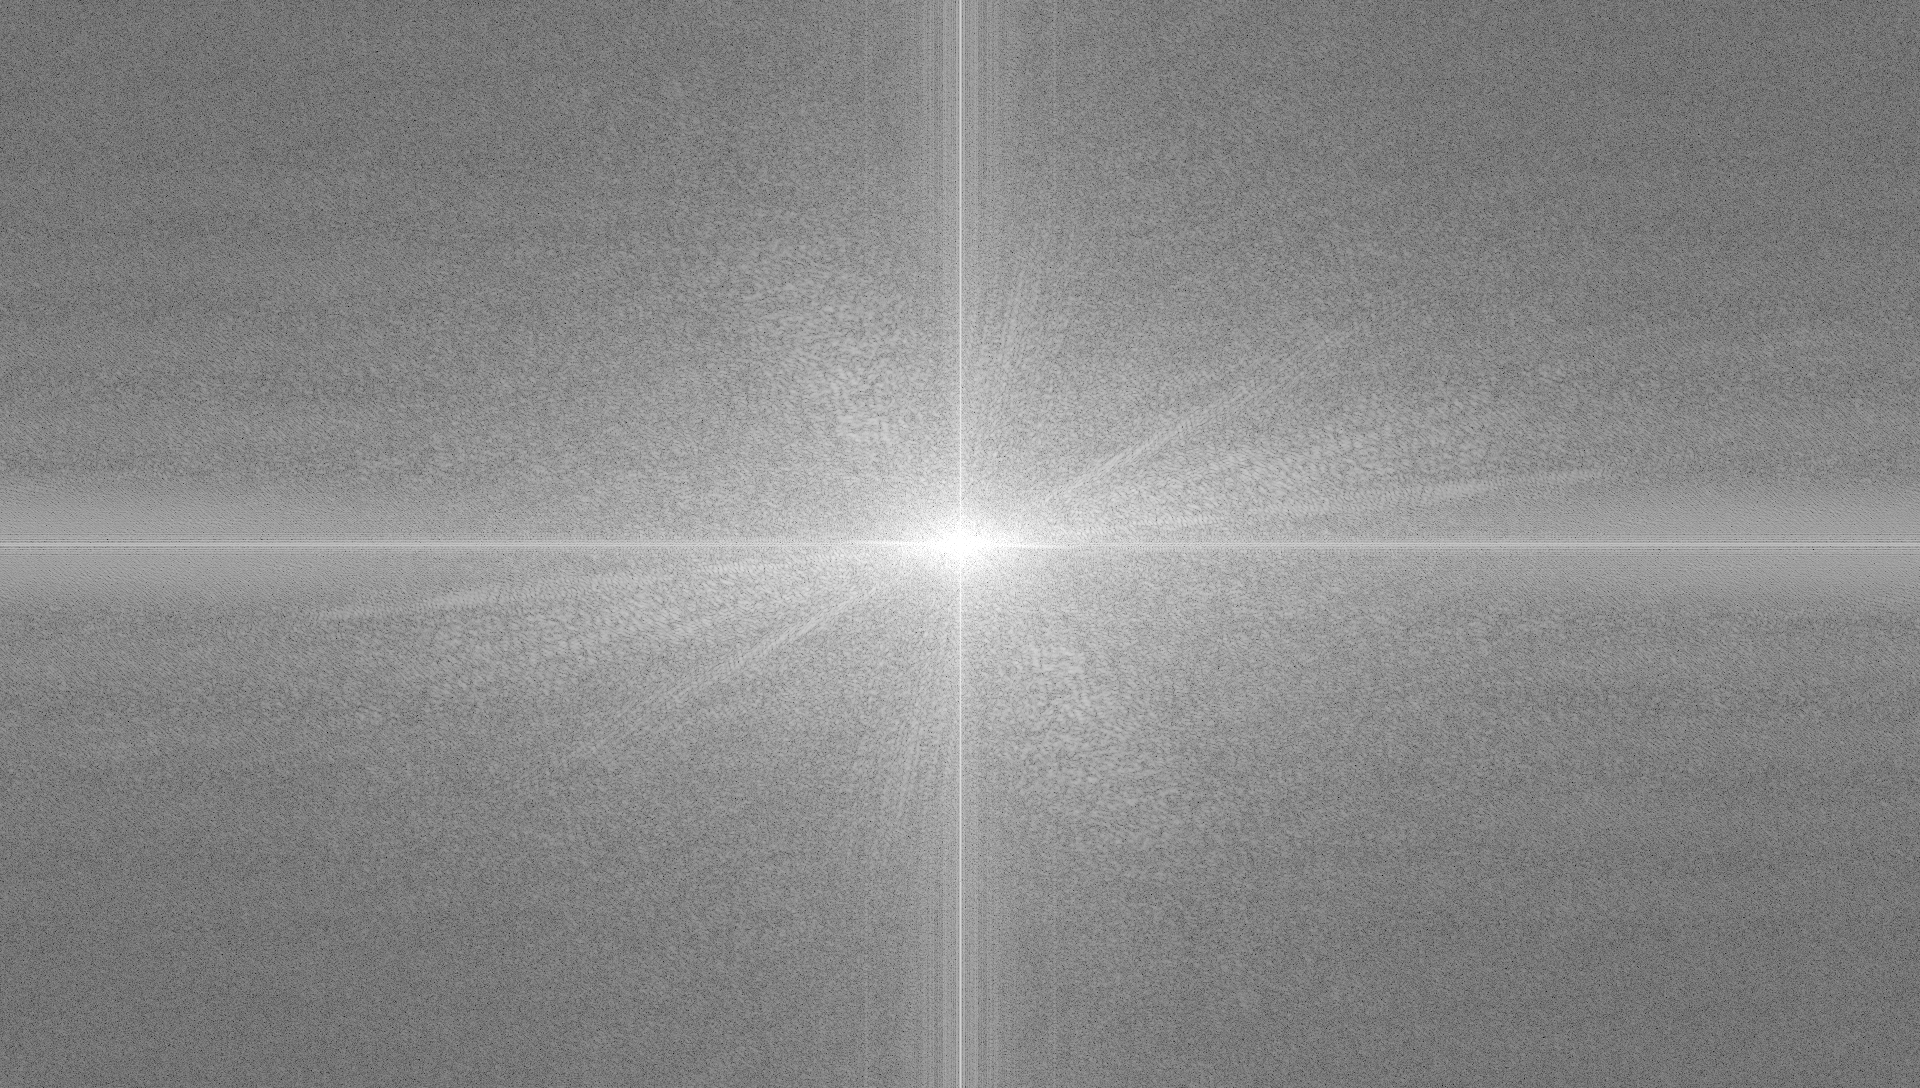
\includegraphics[scale=0.11]{images/bd-14-ft.png}\\\hspace{\fill}\\[-2ex]
\caption[Fourier transform]{Normal image (left) and its DFT (right).}
\label{fig:fourier1}
\end{figure}
\begin{figure}[H]
\centering
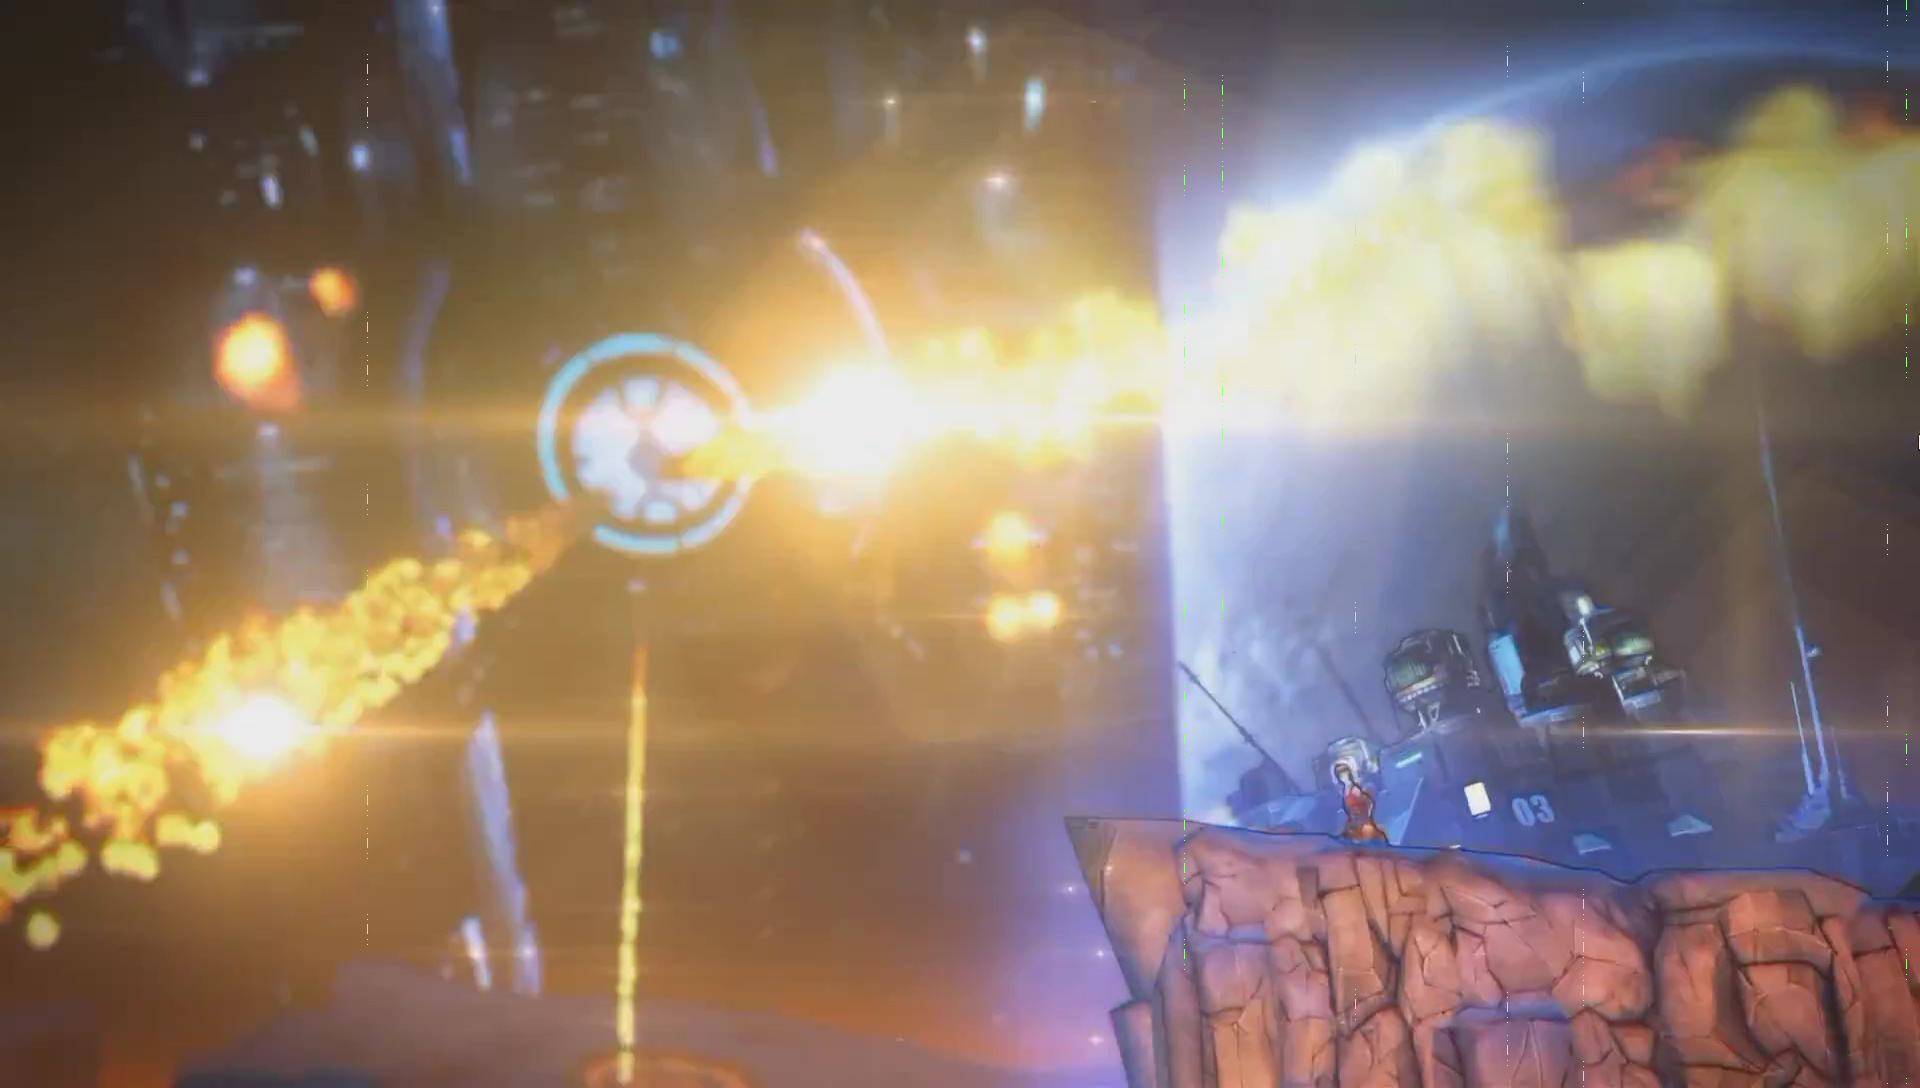
\includegraphics[scale=0.11]{images/experiment10.png}
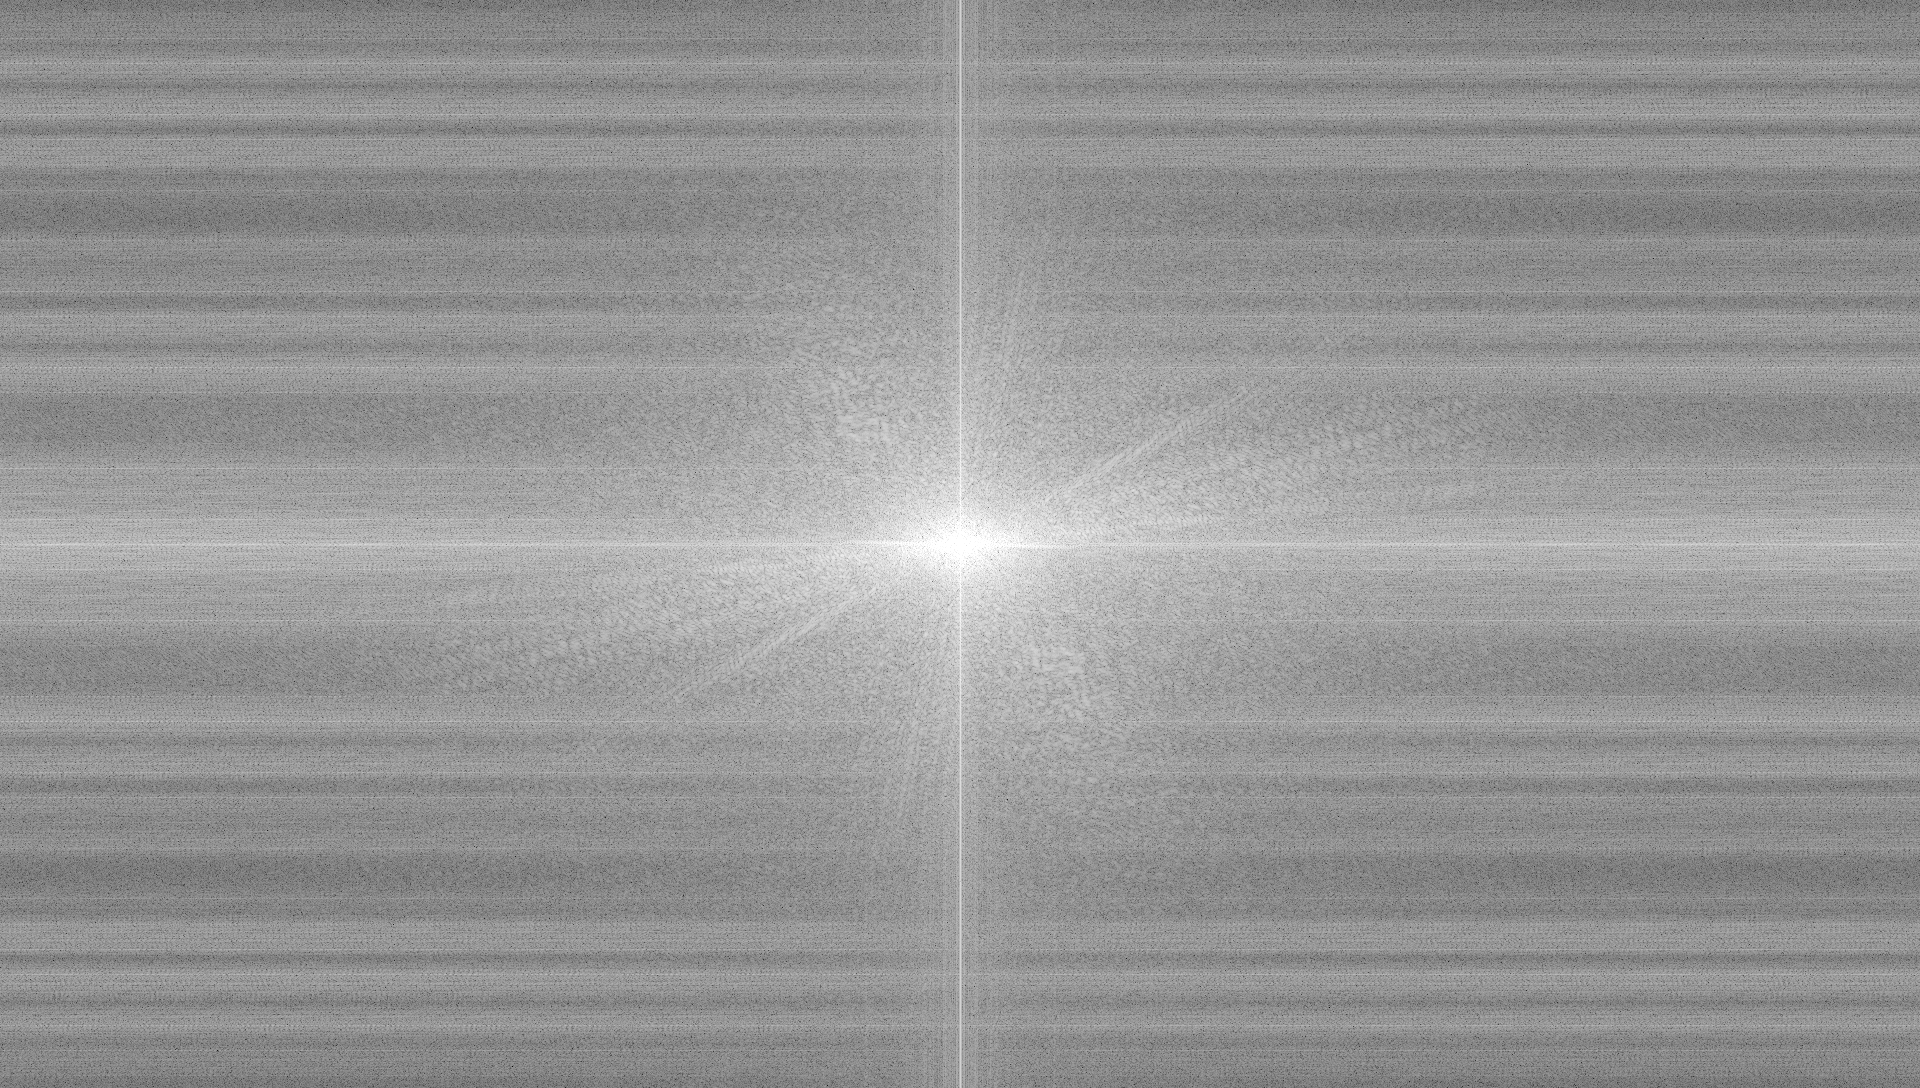
\includegraphics[scale=0.11]{images/experiment11.png}\\\hspace{\fill}\\[-2ex]
\caption[Fourier transform on morse code artifact]{Image with the morse code artifact added (left) and its DFT (right).}
\label{fig:fourier2}
\end{figure}
\begin{figure}[H]
\centering
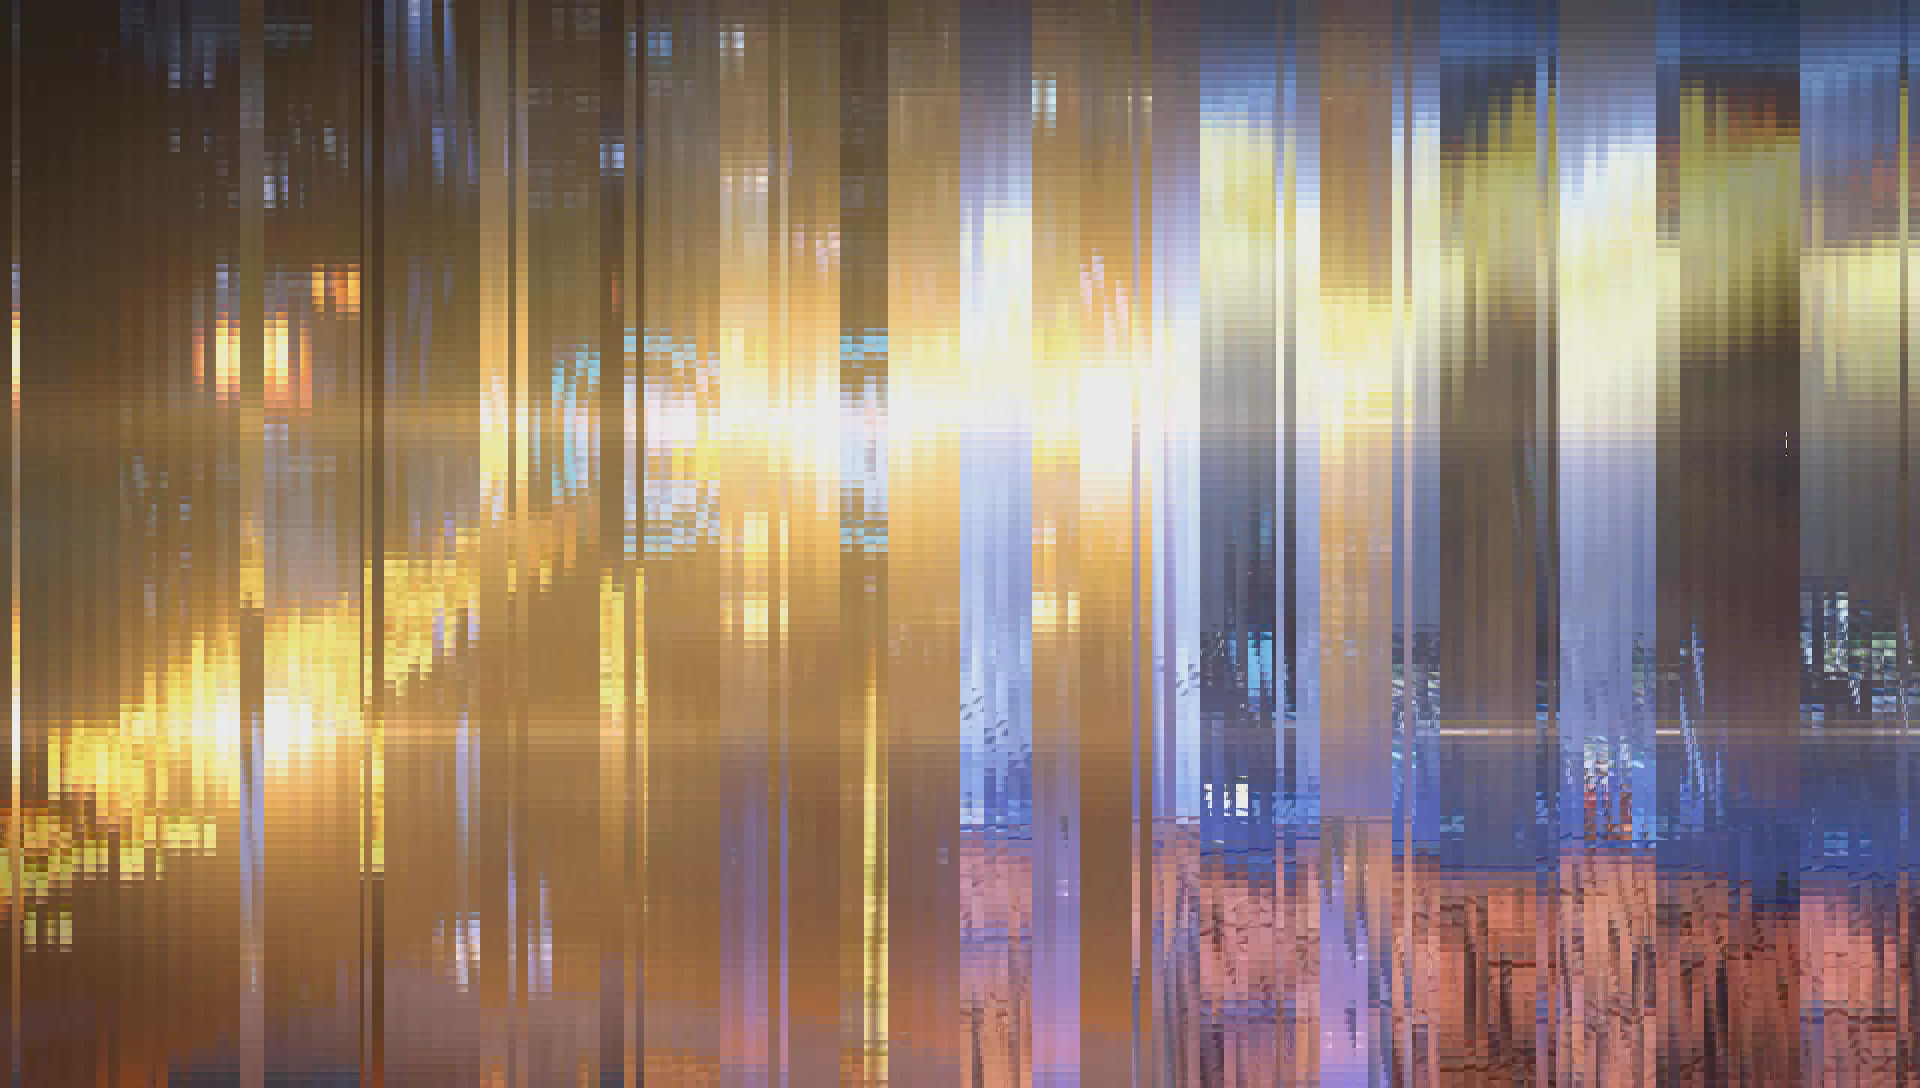
\includegraphics[scale=0.11]{images/0_stuttering.png}
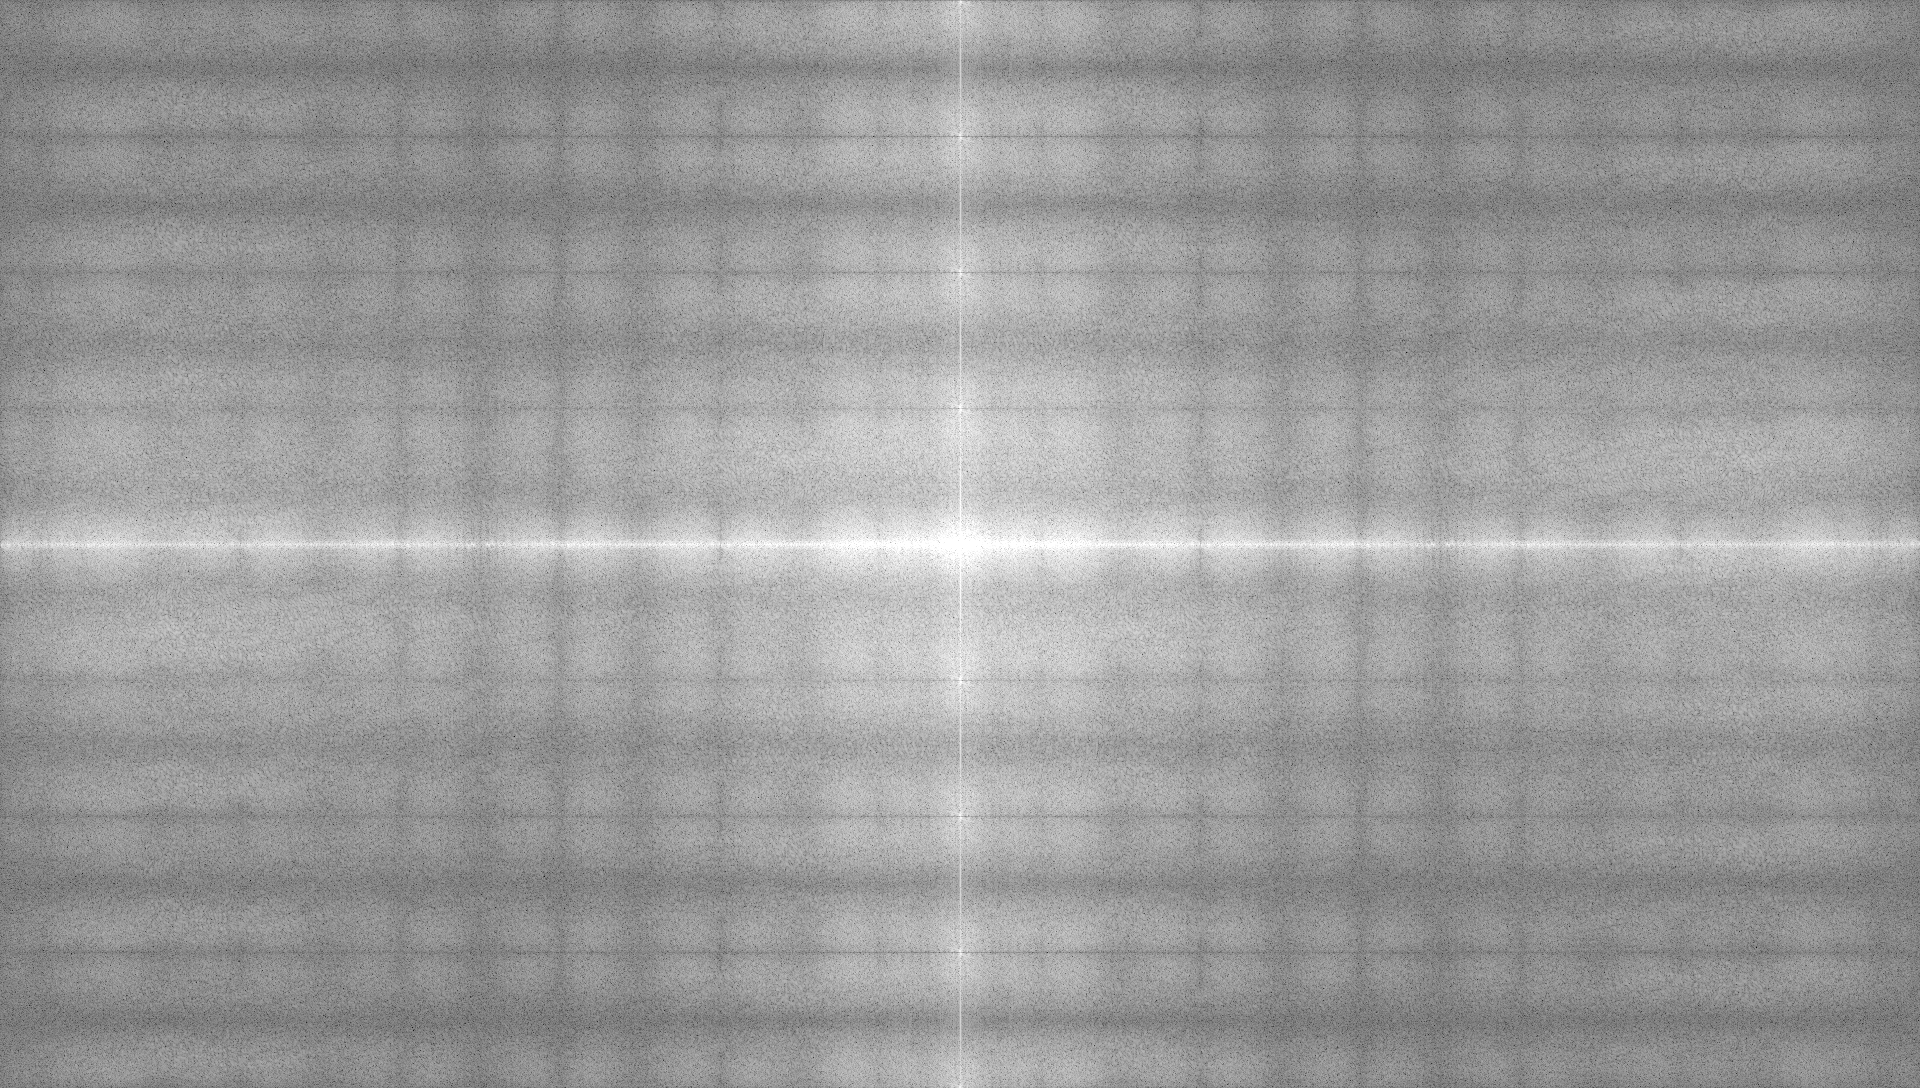
\includegraphics[scale=0.11]{images/stuttering.png}\\\hspace{\fill}\\[-2ex]
\caption[Fourier transform on stuttering artifact]{Image with the stuttering artifact added (left) and its DFT (right).}
\label{fig:fourier4}
\end{figure}
\begin{figure}[H]
\centering
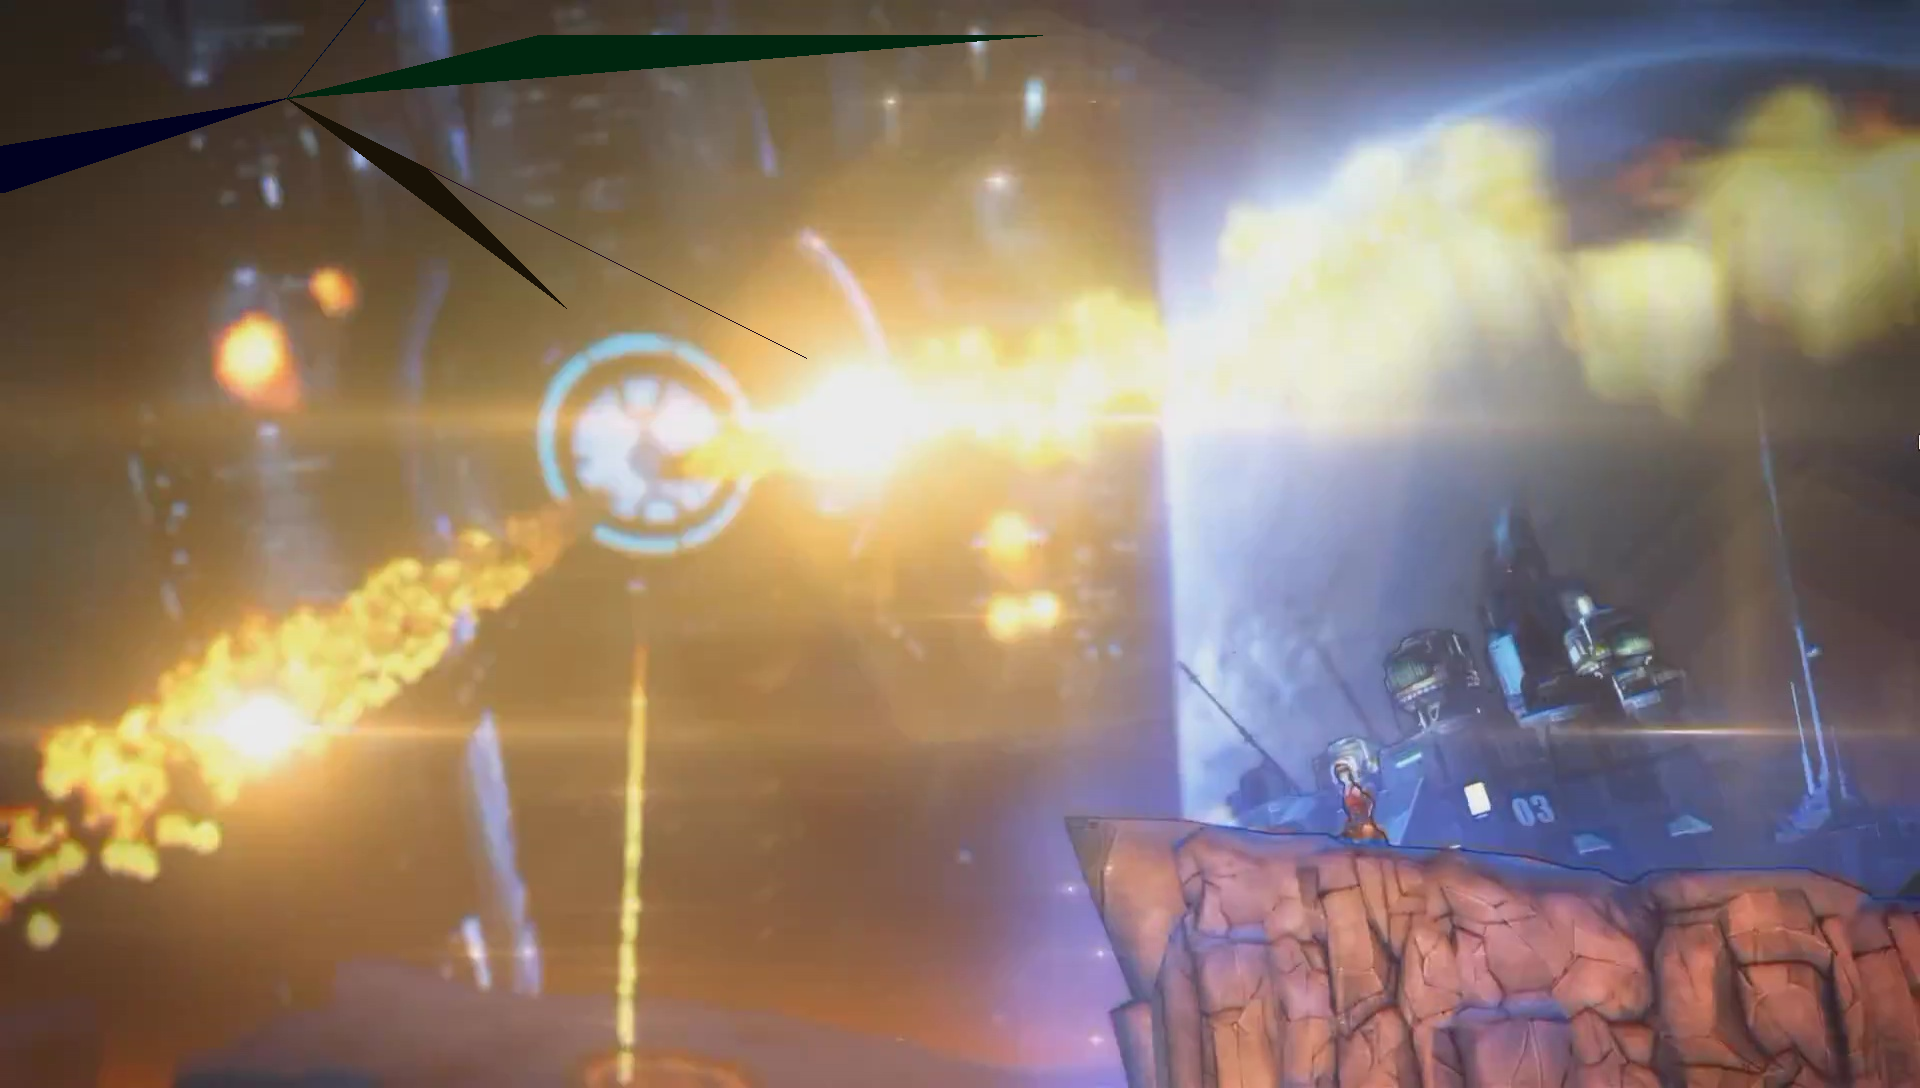
\includegraphics[scale=0.11]{images/0_shape.png}
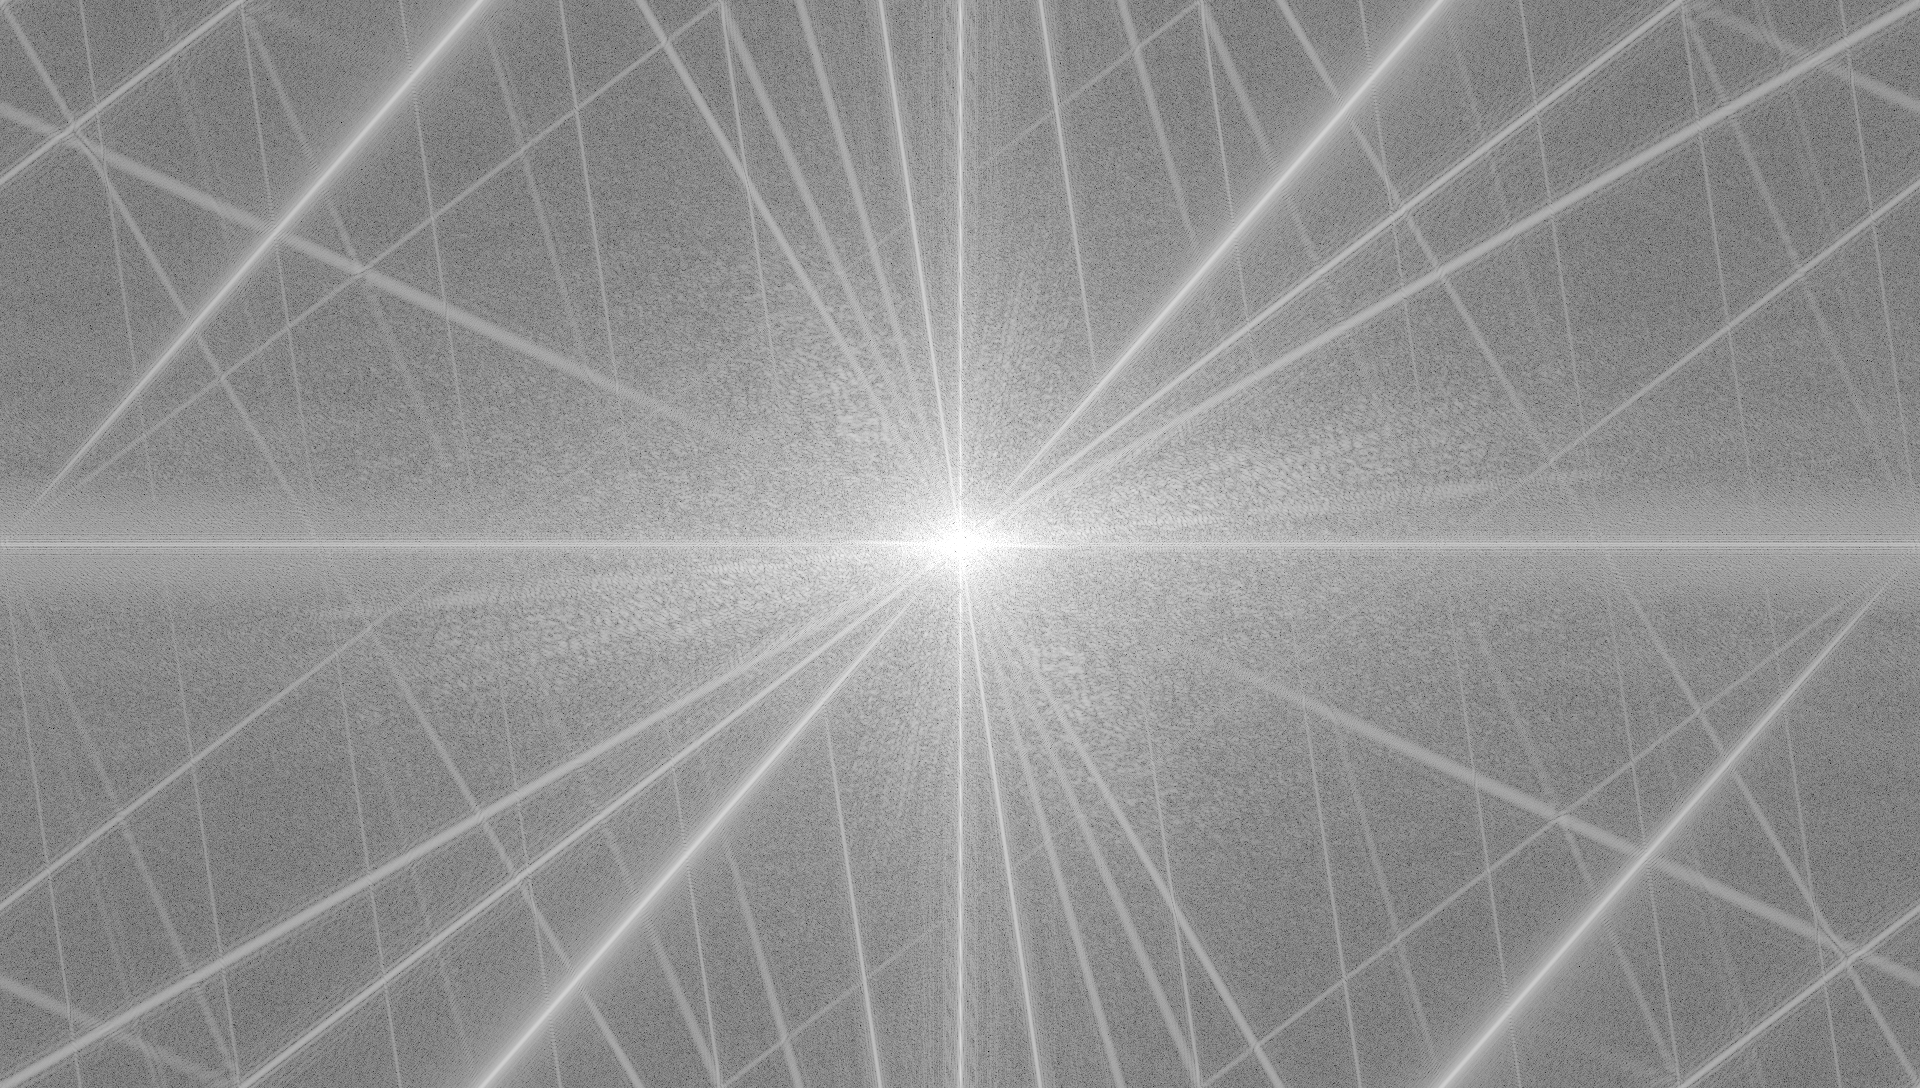
\includegraphics[scale=0.11]{images/shape.png}\\\hspace{\fill}\\[-2ex]
\caption[Fourier transform on stuttering artifact]{Image with the stuttering artifact added (left) and its DFT (right).}
\label{fig:fourier3}
\end{figure}\hspace{\fill}\\
Figure \ref{fig:fourier1} displays an image without defects and its DFT. As seen from Figure \ref{fig:fourier2}, even minor corruptions that are rather imperceptible visually have a substantial effect on the image's DFT. Figures \ref{fig:fourier4} and \ref{fig:fourier3} illustrate the explicit patterns in the image's DFT after other types of artifacts are added to the original frame.\\\hspace{\fill}\\
Most screen artifacts affect the high frequency components of the DFT. Hence, we considered adopting another feature that is constructed from high frequencies of the image spectrum. In particular, we transform the DFT $F(u,v)$ with a high-pass filter to obtain 
\begin{align}
\widetilde{F}(u,v)=\begin{cases} 
      F(u,v) & \lfloor\frac{M}{2}\rfloor-100\leqslant u\leqslant \lfloor\frac{M}{2}\rfloor+100, \lfloor\frac{N}{2}\rfloor-100\leqslant v\leqslant \lfloor\frac{N}{2}\rfloor+100 \\
      0 & \text{otherwise},
   \end{cases}
\end{align}
where original coordinates $0\leqslant u\leqslant M-1$ and $0\leqslant v\leqslant N-1$ are used. The resulting signal $\widetilde{F}(u,v)$ is then brought back to spatial domain to become our new feature $\widetilde{f}(x,y)$  (see Figures \ref{fig:fourier5}, \ref{fig:fourier6}).
\begin{figure}[H]
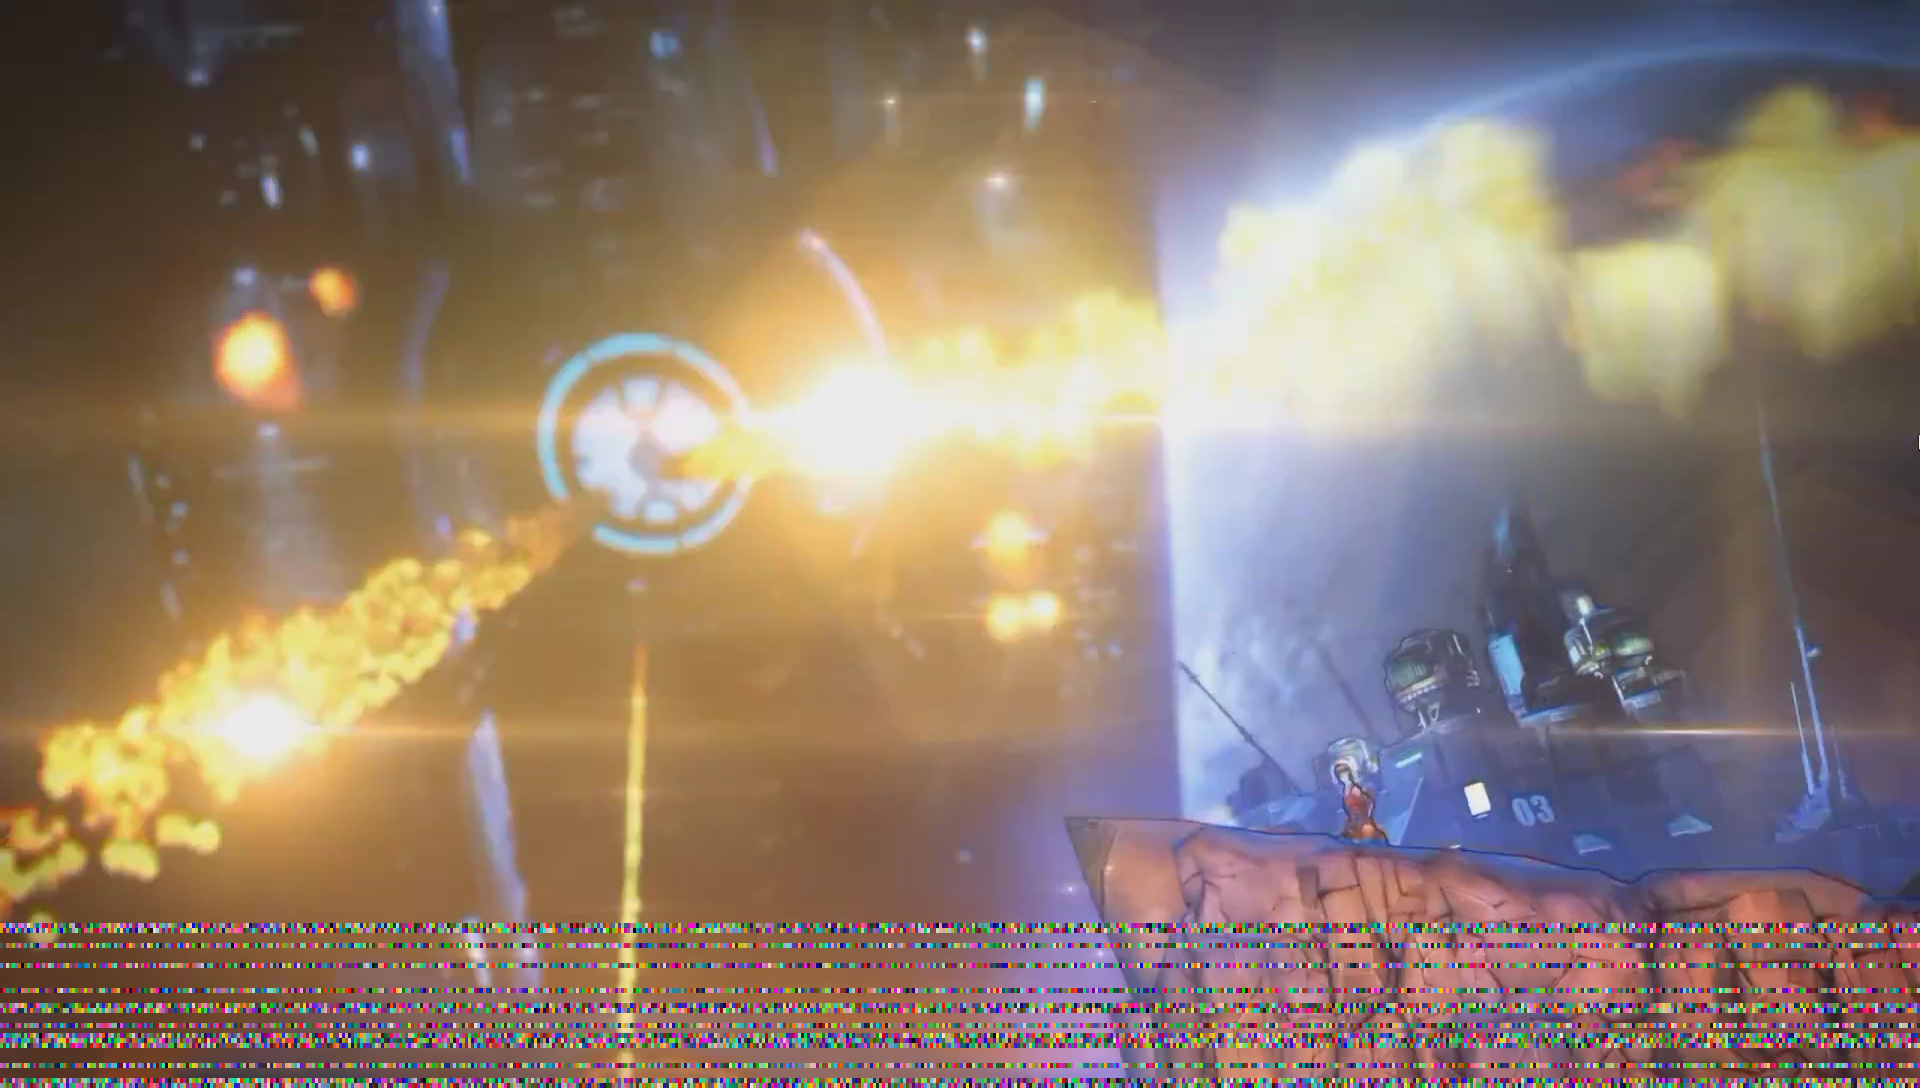
\includegraphics[scale=0.11]{images/pixelationv1.png}
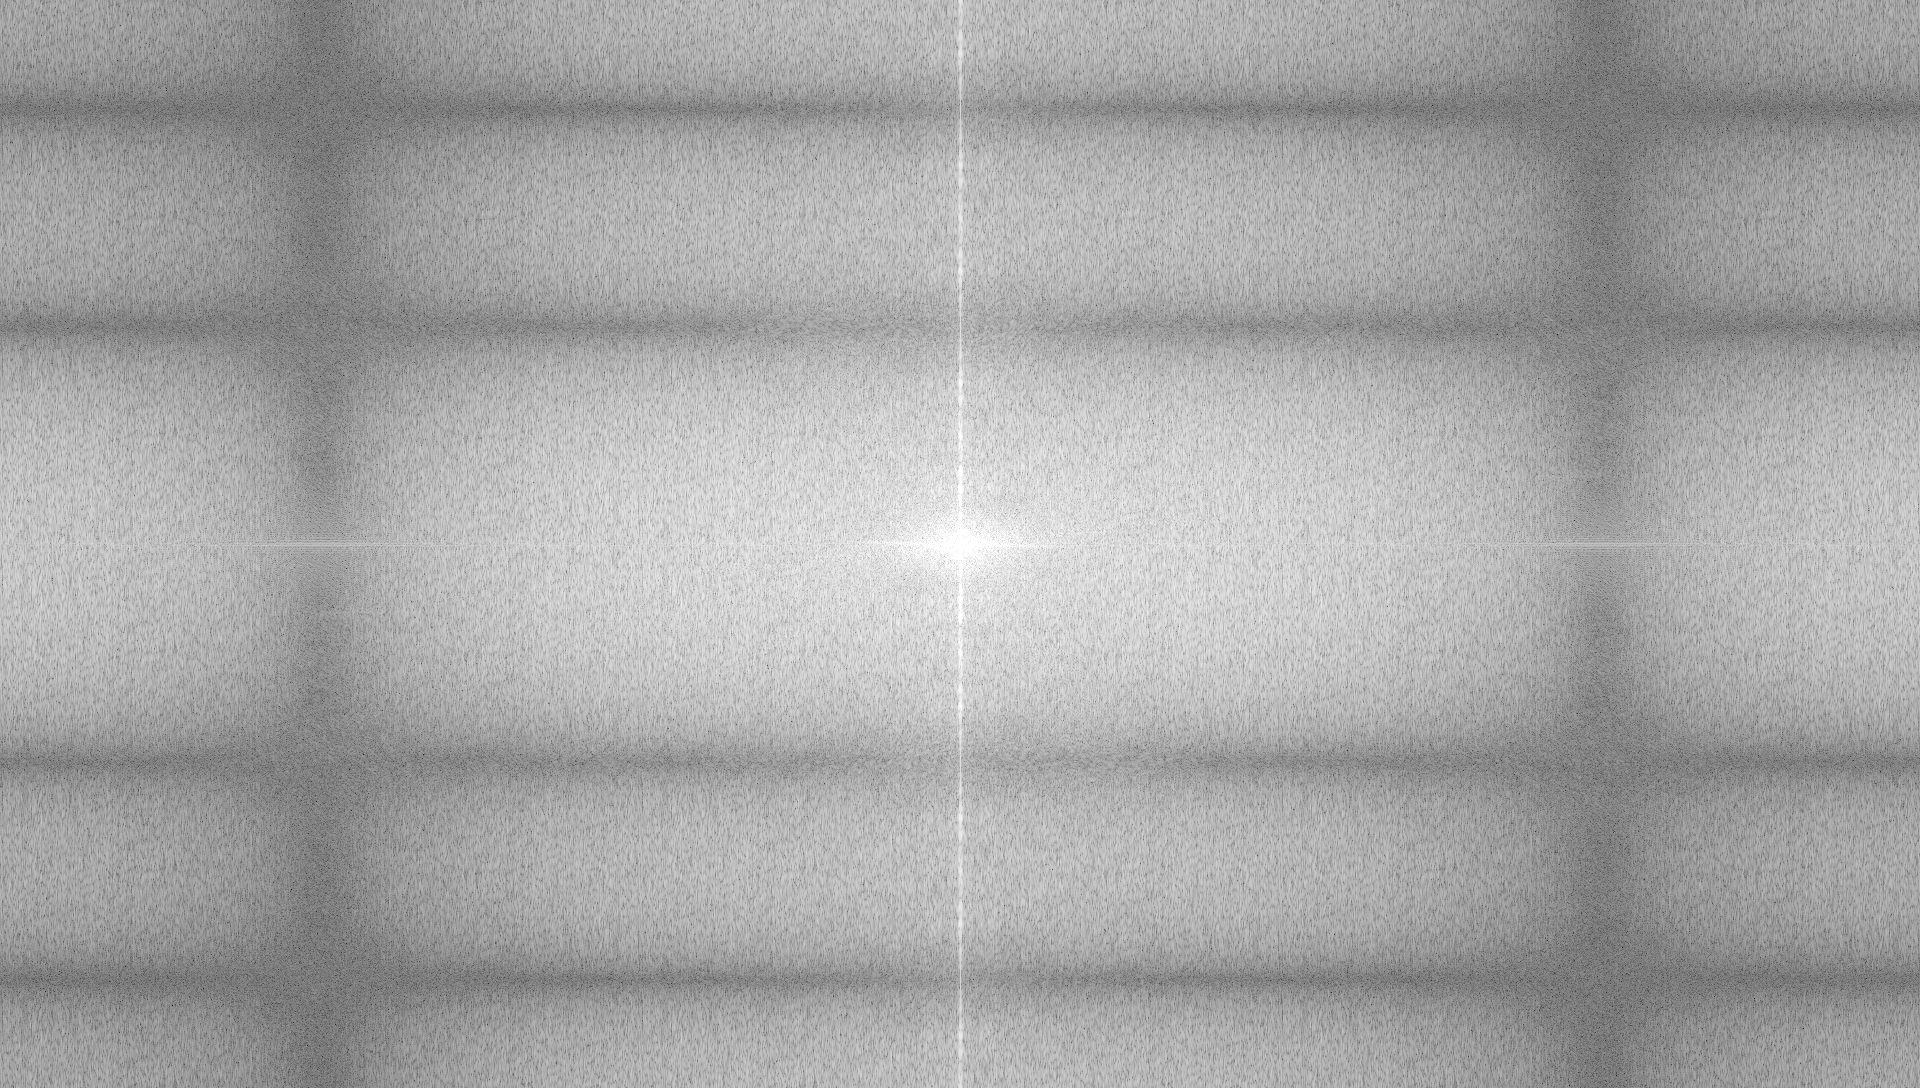
\includegraphics[scale=0.11]{images/pixv1-ft.png}\\
\caption[Fourier transform on stuttering artifact]{Corrupted image $f(x,y)$ (left) and its DFT $F(u,v)$ (right).}
\label{fig:fourier5}
\end{figure}
\begin{figure}[H]
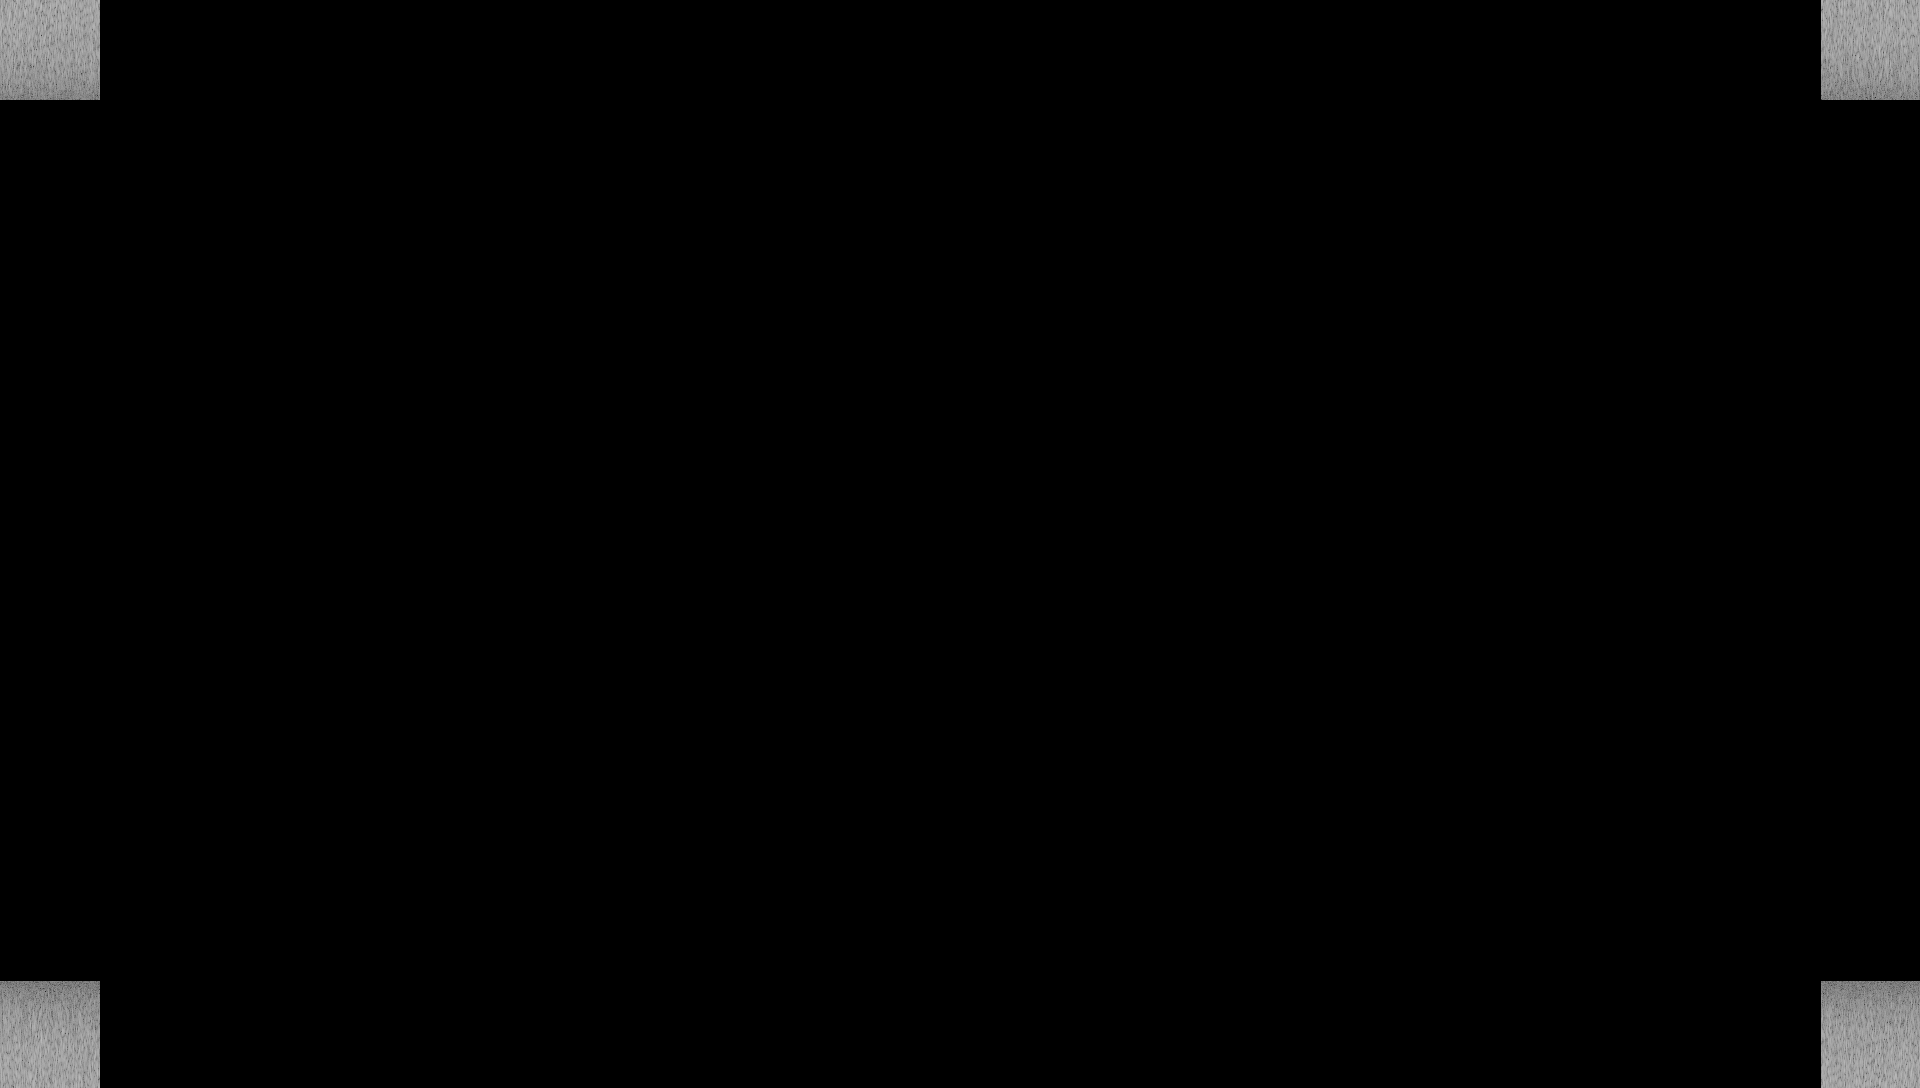
\includegraphics[scale=0.11]{images/pixv1-corn.png}
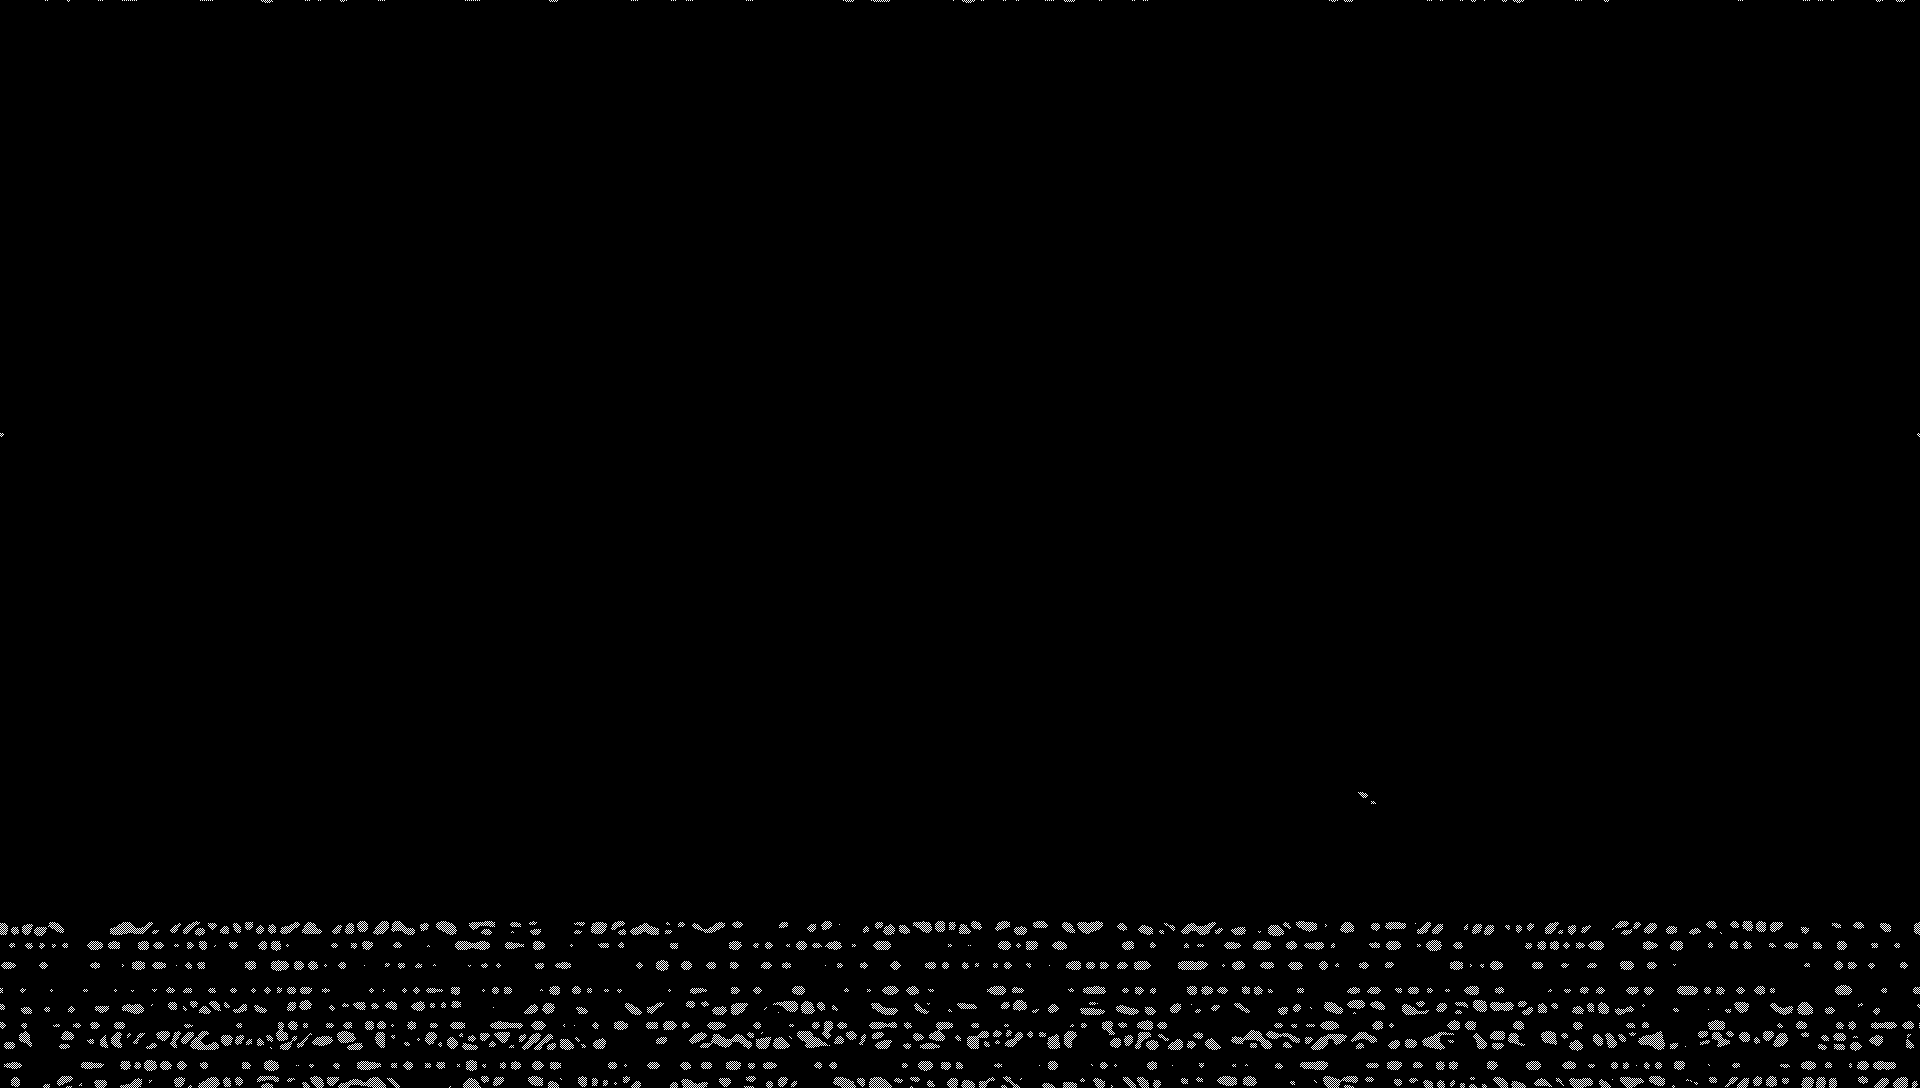
\includegraphics[scale=0.11]{images/pixv1.png}\\
\caption[Fourier transform on stuttering artifact]{High-pass filtered DFT $\widetilde{F}(u,v)$ and its inverse $\widetilde{f}(x,y)$ (right).}
\label{fig:fourier6}
\end{figure}

% Talk about high frequencies and the other feature.

\section{Histogram of Oriented Gradients (HoG)}

Histogram of oriented gradients is a feature used in computer vision to detect objects in an image \cite{1467360}. The steps to compute the HoG feature are shown as follows:\\


\noindent An $M \times N$ color image can be represented using three functions $R,G,B : \mathbb{R}^{M \times N} \rightarrow R$ that map each coordinate to the corresponding red, green, and blue color intensity value, respectively. The gradient of the functions at each coordinate can be approximated by applying discrete derivative masks $[-1,0,1]$ and $[-1,0,1]^T$ at each coordinate. Sometimes different derivative masks such as the Sobel filters (shown in figure \ref{sobel}) are convolved with the image to get a more accurate approximation of the gradients \cite{Gupta2013SobelED}.
\begin{figure}[H]
\centering
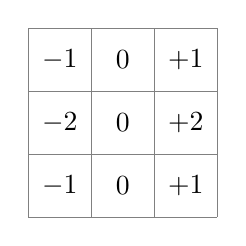
\begin{tikzpicture}
\draw[step=0.8cm,color=gray] (0,0) grid (2.4,2.4);
\node at (0.4,0.4) {$-1$};
\node at (1.2,0.4) {$0$};
\node at (2,0.4) {$+1$};
\node at (0.4,1.2) {$-2$};
\node at (1.2,1.2) {$0$};
\node at (2,1.2) {$+2$};
\node at (0.4,2) {$-1$};
\node at (1.2,2) {$0$};
\node at (2,2) {$+1$};
\end{tikzpicture}
\qquad
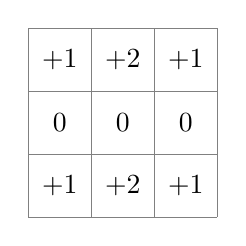
\begin{tikzpicture}
\draw[step=0.8cm,color=gray] (0,0) grid (2.4,2.4);
\node at (0.4,0.4) {$+1$};
\node at (1.2,0.4) {$+2$};
\node at (2,0.4) {$+1$};
\node at (0.4,1.2) {$0$};
\node at (1.2,1.2) {$0$};
\node at (2,1.2) {$0$};
\node at (0.4,2) {$+1$};
\node at (1.2,2) {$+2$};
\node at (2,2) {$+1$};
\end{tikzpicture}\hspace{\fill}\\\hspace{\fill}\\[-2ex]
\caption[Sobel Filters]{Sobel filters along horizontal axis (left) and vertical axis (right).}
\label{sobel}
\end{figure}
%Sobel Filters, which includes a weighted sum of neighboring pixels' gradients to approximate the gradient at the centering pixel
\noindent The image is then divided into small patches, and the magnitude and orientation of gradients within each patch are computed. After that, a histogram of gradients is computed, which contains 9 bins corresponding to angles 0, 20, 40 $\ldots$ 160. For each gradient, bins are selected based on its orientation, and the value that goes to the bins is based on the magnitude of the gradient. For instance, suppose a gradient has a magnitude of 3 and angle of 46 degrees. Since 46 is between 40 and 60, we select the two bins corresponding to 40 and 60 degrees. Now, since the difference between 46 and 40 is 6, and the difference between 46 and 60 is 14, the magnitude that goes to the bin corresponding to 40 degrees is $3 \times \frac{6}{20} = 0.9$, and the magnitude that goes to the bin corresponding to 60 degrees is $3 \times \frac{16}{20} = 2.4$. In this way, a histogram is computed to summarize the gradients within each patch.\\

\noindent Finally, we normalize the histograms and then concatenate them together to form a feature descriptor of the entire image. As indicated in figure \ref{visualization of HoG}, HoG serves as an edge detector of objects presented in an image \cite{7025824}.

\begin{figure}[h]
\captionsetup{justification=centering}
    \centering
    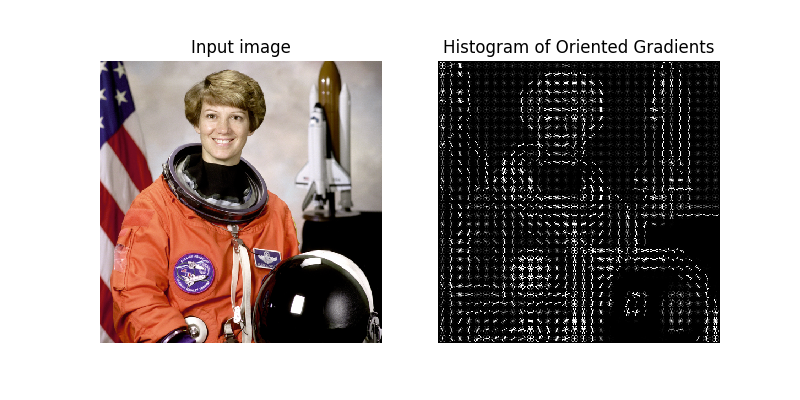
\includegraphics[scale=0.6]{images/hog_vis.png}
  % \centering
    \caption{Visualization of HoG.}
    \label{visualization of HoG}
\end{figure}

% \subsection{Graph Laplacian}

\section{Principal Component Analysis (PCA)}

Principal component analysis (PCA) is a commonly used dimensionality reduction technique in machine learning and statistics \cite{pca_reduction}. It attempts to find linear combinations of features in the original high dimensional data matrix to construct meaningful representation of the dataset \cite{doi:10.1080/14786440109462720}. 


\subsection{Definition}

\noindent 
Suppose the data consists of $n$ $m$-dimensional mean-centered examples $x^{(1)}, x^{(2)}, \ldots, x^{(n)}$ with $x^{(i)} \in \mathbb{R}^{m}$ $\forall i = 1,2, \ldots, n$. \\

\noindent
For any $k \in \{1,2, \ldots,  n\}$ and any set of orthonormal vectors $  u_1, u_2, \ldots, u_k \in  \mathbb{R}^{m}$, define the reconstruction error of the set of vectors as $$ \text{Err} (\{ u_1, u_2, \ldots, u_k\}) =  \sum_{i=1}^{n} || x^{(i)} - {  \hat{x}^{(i)}  }||_2^2$$ where $$\hat{x}^{(i)}   = \sum_{j=1}^{k} (u_i^{T} x^{(i)} )u_i  $$ is the projection of $x^{(i)} $ onto the subspace spanned by the given set of vectors.\\

\noindent The principle components (PCs) of the dataset are defined iteratively:

\noindent
The first PC $v_1$ is given by $$v_1 =  \text{argmin}_{||v||_2 =  1}  \text{Err} (\{v\}) $$

\noindent
For any $k \in \{1,2,\ldots, n-1\}$, after the first $k$ PCs $v_1, \ldots, v_k$ are determined, the $(k+1)^{th}$ PC is given by $$ v_{k+1} =  \text{argmin}_{||v||_2 =  1, v \perp v_i \; \forall i =1,2, \ldots, k}  \text{Err} (\{v_1, v_2, \ldots, v_k, v\}) $$


\subsection{Singular Value Decomposition (SVD)}
Formally, the SVD of a matrix $X \in \mathbb{R}^{n \times m}$ is a factorization of the form $X$ = $U \Sigma V^{T}$, where $U \in \mathbb{R}^{n \times n}, V \in \mathbb{R}^{m \times m}$ are orthonormal matrices, and $\Sigma \in \mathbb{R}^{n \times m}$ is a diagonal matrix consisting of non-negative entries.\\



\noindent SVD is often used to compute the principal components of a given dataset \cite{pca_via_svd}.  According to the following proposition, the principle components are exactly the right singular vectors of the matrix $X$, where $$X = [x^{(1)} \; x^{(2)} \ldots \; x^{(n)} ]^T$$
\noindent \begin{prop} \label{5.1}
Given any mean centered dataset $ x^{(1)}, x^{(2)}, \ldots, x^{(n)} \in \mathbb{R}^{m}$. The $k^{th}$ PC $v_k$ is the $k^{th}$ normalized right singular vector of $X$.
\end{prop}



\noindent The proposition allows us to efficiently compute the principle components of any given dataset using SVD algorithms. However, computing the exact value of SVD takes $O(mn \min (m,n))$ time, and the operations are not parallelizable. Therefore, it is not feasible when the values of $m$ and $n$ are large. Therefore, we also uses randomization techniques to trade accuracy for shorter run time:

\subsection{Randomized SVD}

\noindent Given any real matrix $X$ of dimension $n \times m$, the randomized power iteration SVD algorithm works as follows \cite{randomized_svd,random_svd2}:\\



        \noindent 1. Pick some small positive integers $k$, $p$, and $q$. Sample a matrix $\Omega$ of dimension $n \times (k+p)$, whose entries are IID standard normal.\\

 \noindent 2. Compute an SVD for $(XX^T)^{q}X\Omega  = Q DR$, and only keep the first $t$ columns of matrix $Q$, where $ t \leq k+p$ is the column rank of $D$.\\

 \noindent 3. Compute an SVD for $Q^T X = T \widetilde{ \Sigma} \widetilde{ V}^T$. Compute $\widetilde{U}= QT$, and return $\widetilde{ U} \widetilde{ \Sigma} \widetilde{ V}^T$ as an approximate SVD for $X$.\\
 
 
 


 \noindent Runtime of the algorithm is $O(mn \min (m,n))$, which is the same as that of the deterministic algorithm. However, since the most expensive operations in this algorithm are matrix multiplications, the algorithm can easily be parallelized, which results in a much shorter runtime. Furthermore, we can show that the expected approximation error of this algorithm approaches the optimal value as the value of $q$ increases:
 
 
\begin{theorem}Select a target rank $k \geq 2$ and an oversampling parameter $p \geq 2$. For any real matrix $X \in \mathbb{R}^{n \times m}$, select any integer $q \geq 0$ and execute the randomized power iteration SVD algorithm. Then
\begin{align*}
\mathbb { E } \left \| X - \widetilde{ U} \widetilde{\Sigma} \widetilde{V}^{T} \right\|_2 \leq \left [ \left( 1 + \sqrt { \frac { k } { p - 1 } } \right) \sigma _ { k + 1 }^{2q+1} + \frac { \mathrm { e } \sqrt { k + p } } { p } \left( \sum _ { j > k } \sigma _ { j } ^ { 2 (2q+1)} \right) ^ { 1 / 2 } \right ]^{\frac{1}{2q+1}}\tag{4.3} \label{Eq 4.3}
\end{align*}
\noindent where $\sigma_{j}$ is the $j^{th}$ singular value of $X$ $\forall j = 1,2, \ldots, n$.
\end{theorem}


\noindent If we bound the series in the inequality \ref{Eq 4.3} using its largest term $\sigma_{k+1}^{2(2q+1)}$ and draw the factor $\sigma_{k+1}$ out of the bracket, then
$$\mathbb { E } \left \| X - \widetilde{ U} \widetilde{\Sigma} \widetilde{V}^{T} \right\|_2 \leq \left[ 1 + \sqrt { \frac { k } { p - 1 } } + \frac { \mathrm { e } \sqrt { k + p } } { p } \cdot \sqrt { \min \{ m , n \} - k } \right] ^ { 1 / ( 2 q + 1 ) } \sigma _ { k + 1 }$$

\noindent
As $q$ becomes larger, the expression on the right approaches $ \sigma_{k+1}$, which is the smallest possible approximation error for any rank-$  k $ matrix.\\


\noindent In conclusion, the randomized SVD algorithm enables us to compute a close approximation of the singular value decomposition for any real matrix within a relatively short amount of time. Hence we use this algorithm to reduce the dimensionality of our data.

 
 
 
\section{Pixel-wise Anomaly Measure}

\noindent Given an image, we approximate the distribution of red, green, and blue intensities, and then assign each individual pixel an anomaly score based on how much the pixel's intensity deviates from the estimated global distribution \cite{RX_detector}. This process can be done using graph-based method described below \cite{graph_lap} as follows.\\

\noindent Consider an undirected, weighted graph $G = (V,E)$ composed of a vertex set $V =\{r,g,b\}$ corresponding to the three color intensities, and an edge set $E$ specified by $(a, b, w_{ab})$, where $a, b \in V$, and $w_{ab} \in \mathbb{R}^{+}$ is the edge weight between vertices $a$ and $b$.  In our case, the edge weights are defined as:
\begin{align}
w_{rg}=\frac{1}{1+\left(\frac{\mu_{r}-\mu_{g}}{\alpha}\right)^{2}}, w_{rb}=\frac{1}{1+\left(\frac{\mu_{r}-\mu_{b}}{\alpha}\right)^{2}}, w_{gb}=\frac{1}{1+\left(\frac{\mu_{g}-\mu_{b}}{\alpha}\right)^{2}}
\end{align}
\noindent where $\alpha = \frac{\mu_a + \mu_g + \mu_b}{3}$ and $\mu_r, \mu_g, \mu_b$ are the average red, green, and blue intensities in the image, respectively. From the adjacency matrix $W$, the combinatorial graph Laplacian matrix
$L = D - W$ can be computed, where $D$ is the degree matrix defined by:
\begin{align}
D(a, b)=\left\{\begin{array}{ll}{\sum_{k=1}^{n} w_{a k}} & {\text { if } a=b} \\ {0} & {\text { otherwise }}\end{array}\right.
\end{align}\hspace{\fill}\\
\noindent Finally, we normalize the Laplacian matrix $
L^{*}=D^{-\frac{1}{2}}L D^{-\frac{1}{2}}
$ and define an anomaly measure for each pixel $x$ in the image by:
$$ \delta(x) = s^T L^* s,$$
 \noindent where $s \in \mathbb{R}^3$ is the color intensity of $x$.\\





\noindent The anomaly measures can be used to identify anomalous pixels as shown in the figures below:

\begin{figure}[H]
    \centering
    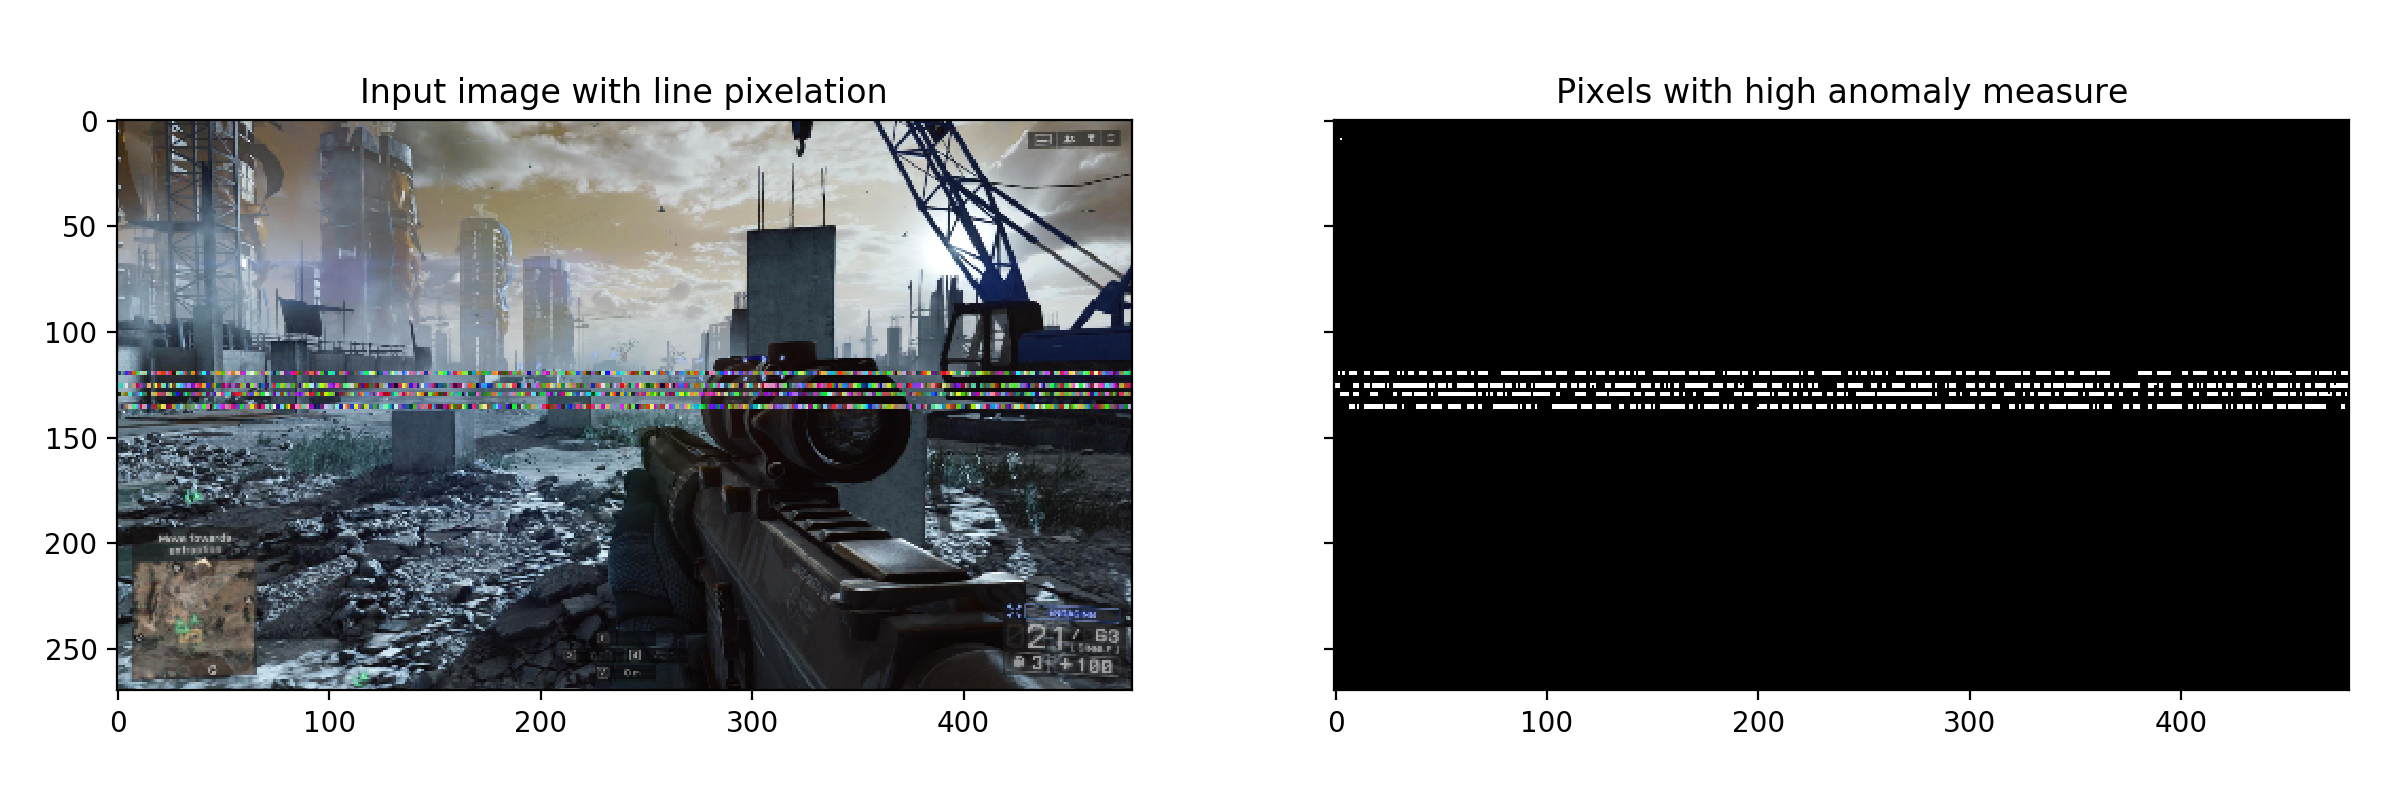
\includegraphics[scale=0.5]{images/graph_laplacian_1.png}
    
    
    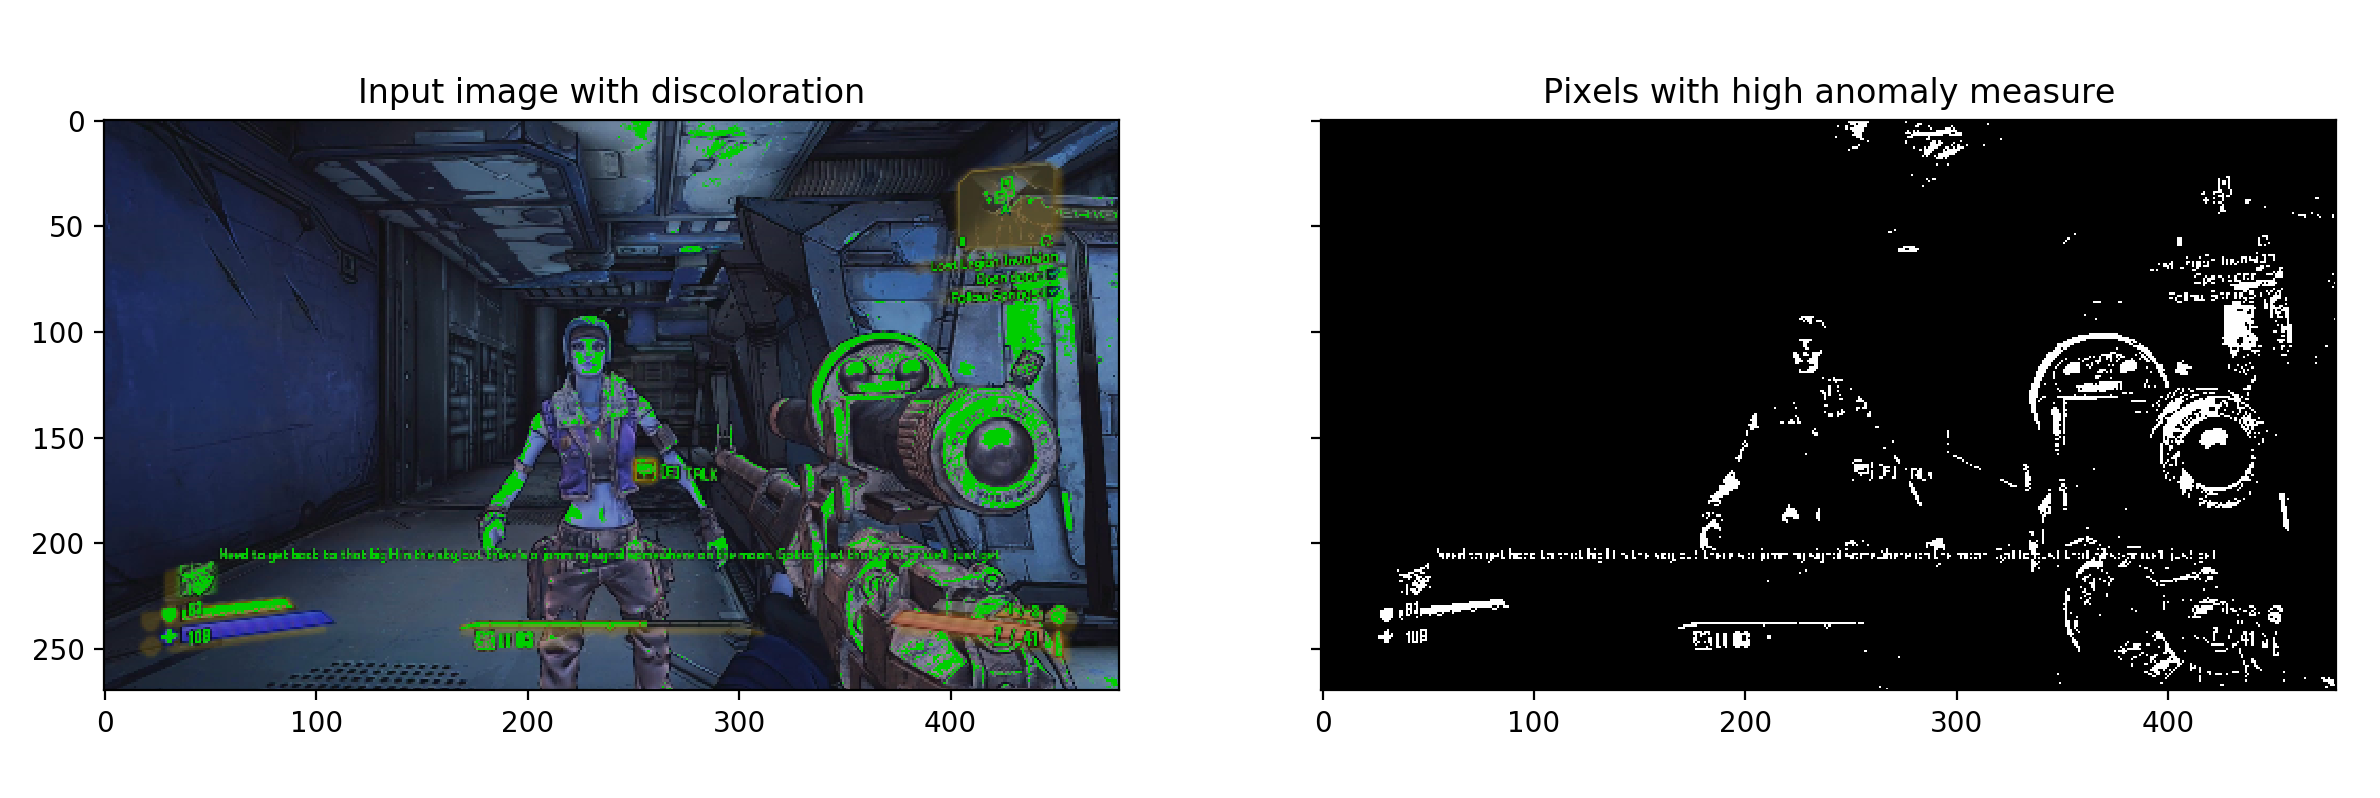
\includegraphics[scale=0.5]{images/graph_laplacian_2.png}
  % \centering
    \caption{Results of the graph-based anomaly detection algorithm.}
    \label{fig:graphlaplacian}
\end{figure}



\noindent The images on the left are examples with artifacts. The binary images on the right are the results of the graph-based anomaly detection algorithm, where pixels in white have anomaly measure exceeding the mean value by at least two standard deviations. As we can see from the figures, most pixelated patches and discolorated pixels have high anomaly scores. \\

\noindent Since corrupted pixels tend to appear together in clusters, we apply dilation to the results of the anomaly detection algorithm to fill in small holes in each cluster \cite{dilation}. Here dilation refers to setting any pixel in a binary image to 1 if any of its neighboring pixels have the value 1. An example is shown in Figure \ref{fig:dilation}.


\begin{figure}[H]
    \centering
    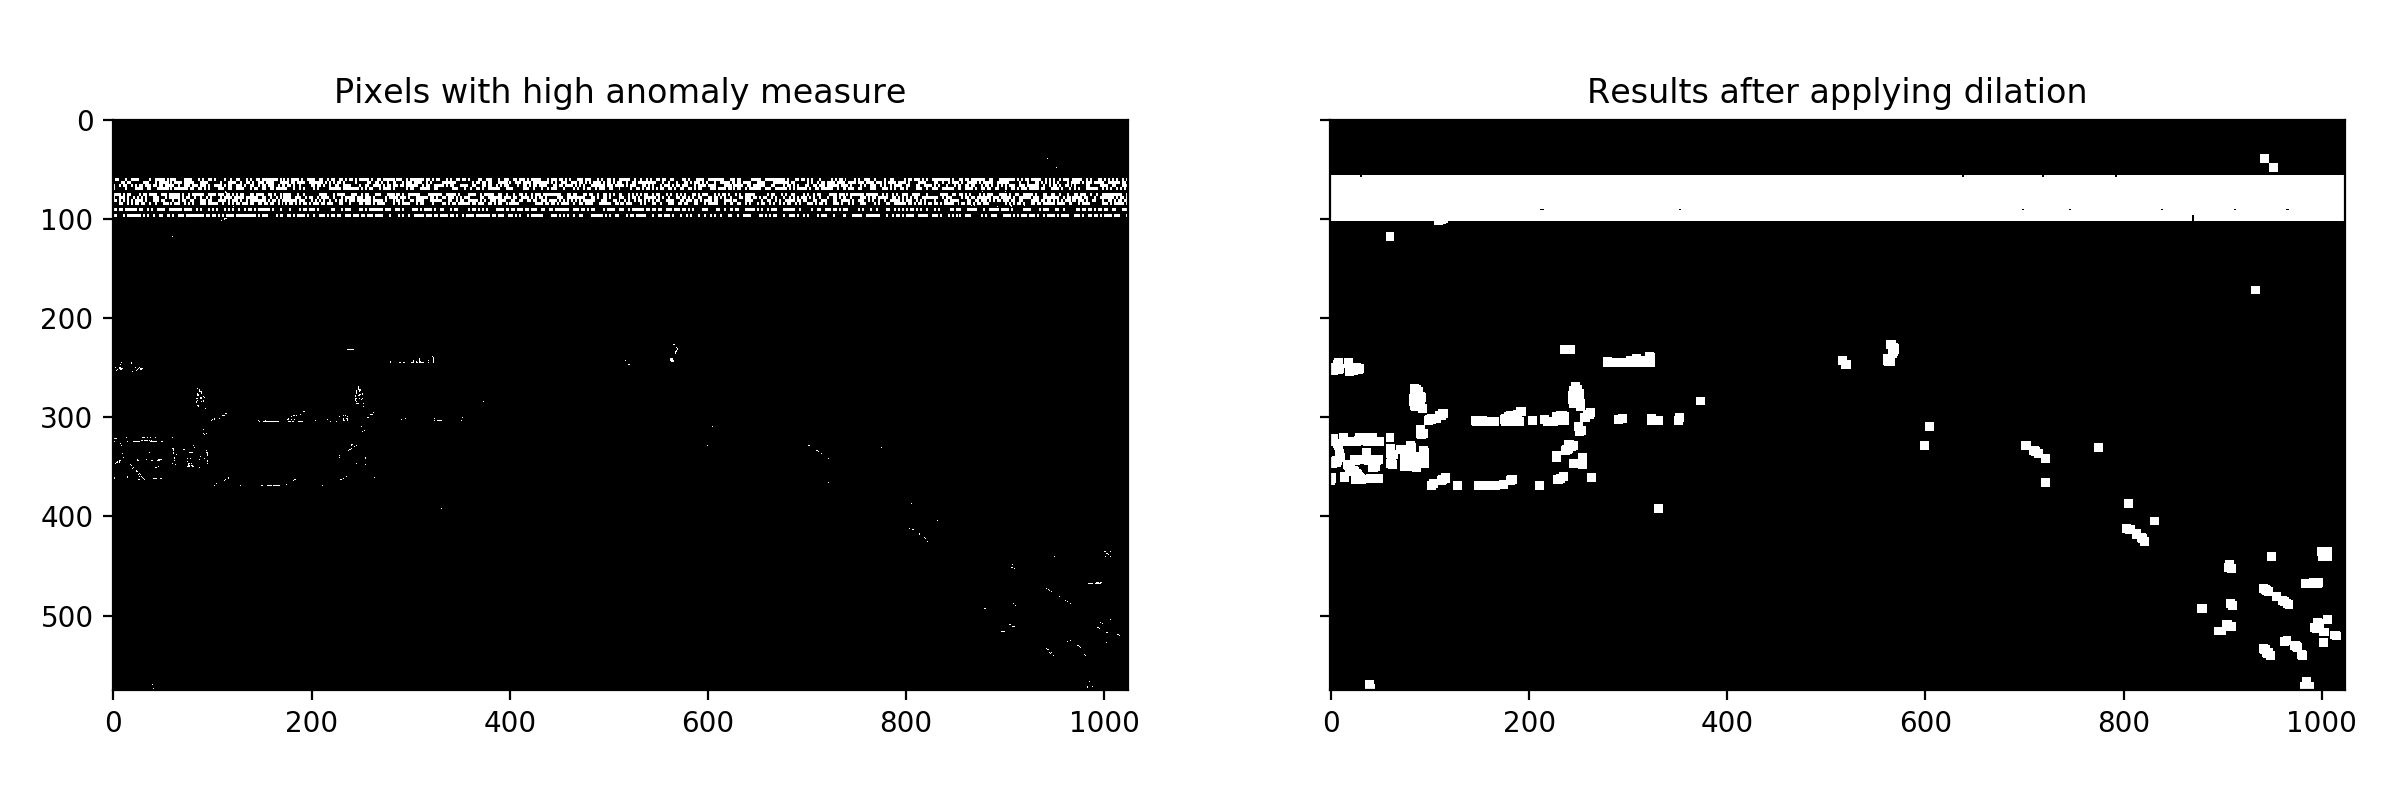
\includegraphics[scale=0.5]{images/dilation.png}
    
    
  % \centering
    \caption{Applying dilation to the results of the graph-based anomaly detection algorithm.}
    \label{fig:dilation}
\end{figure}



\noindent However, sometimes pixels with high anomaly scores are not corrupted, as shown in the figure below. Therefore we combine pixel-wise anomaly measure with other features in order to detect artifacts without producing too many false positives.

\begin{figure}[H]
    \centering
    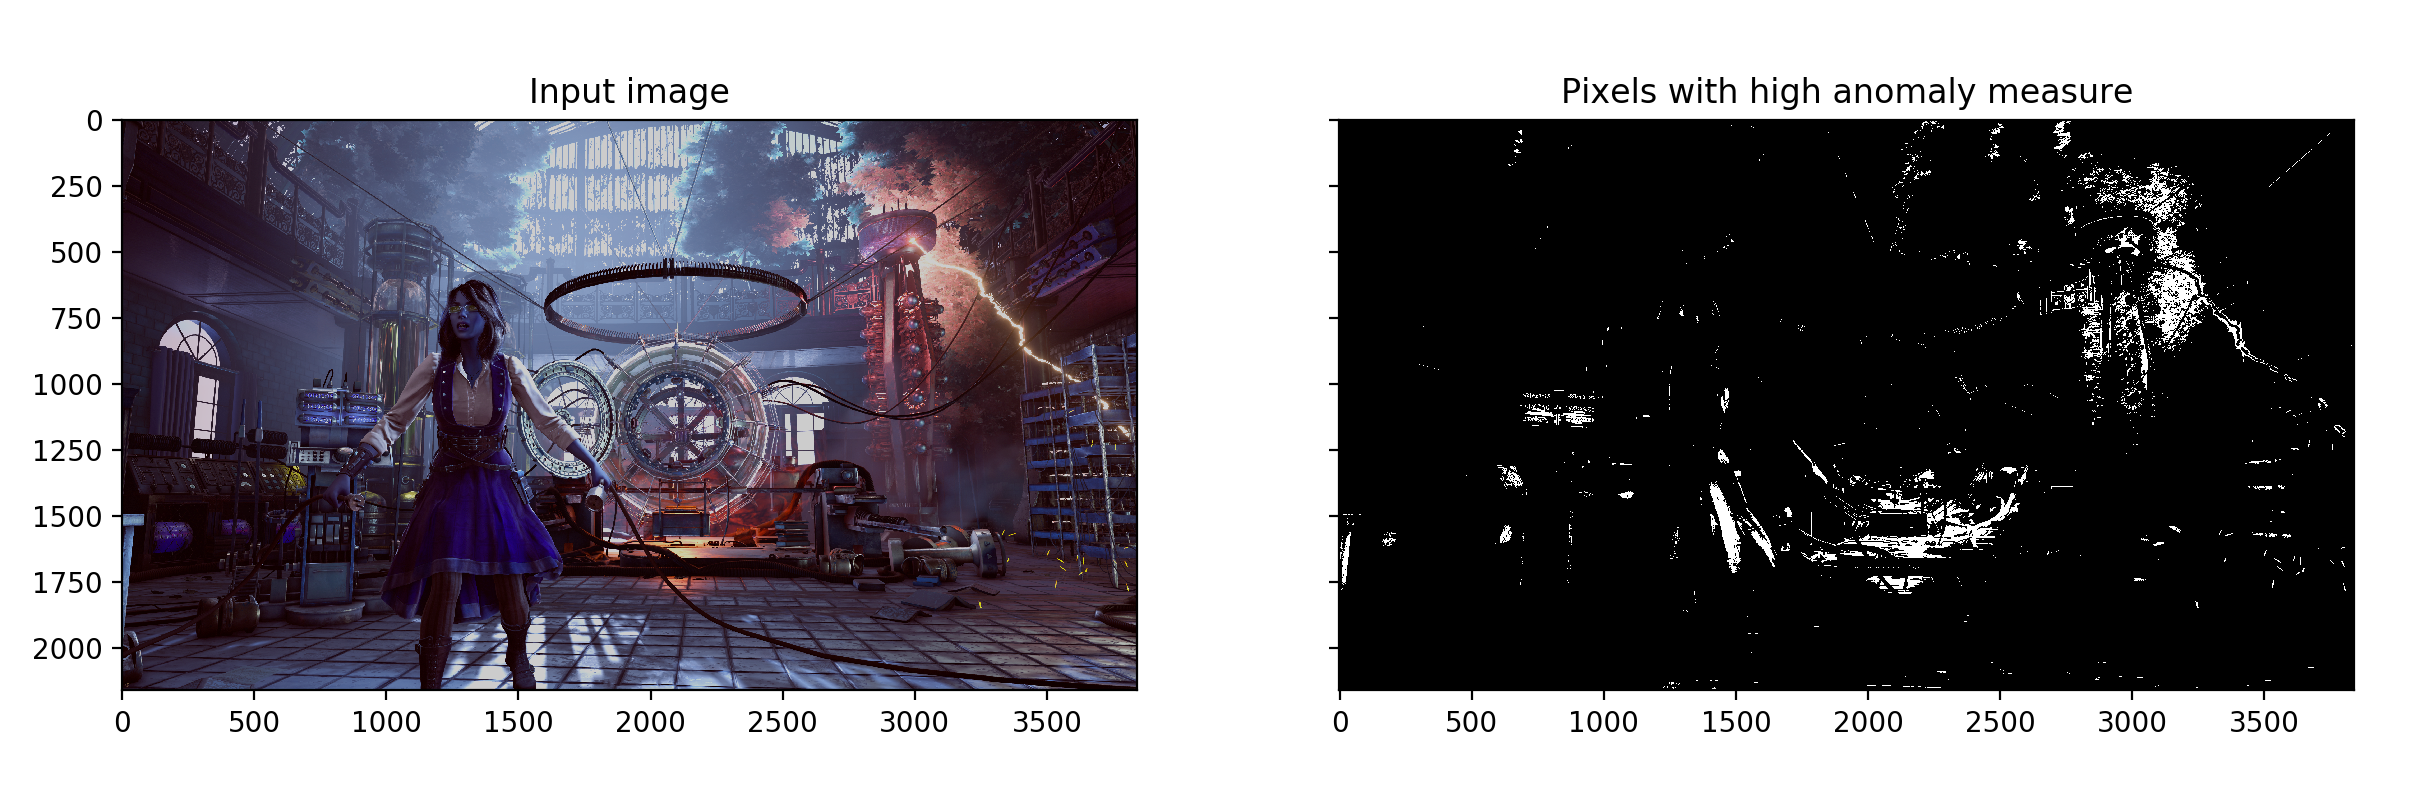
\includegraphics[scale=0.5]{images/graph_laplacian_false_postive.png}
    

  % \centering
    \caption{False positives produced by the graph-based anomaly detection algorithm.}
    \label{fig:graphlaplacianfp}
\end{figure}



\noindent 

\endinput